\documentclass{article}

\usepackage{html}
\usepackage{graphicx}
\usepackage{tikz}

\usetikzlibrary[arrows.meta,backgrounds,calc,fit,positioning,shapes.multipart]

% Also ****ing broken.
%\newenvironment{ezcode}{\begin{quote}\begin{verbatim}}{\end{verbatim}\end{quote}}

\begin{document}

This page contains links to writings about topics such as technology, video games, and philosophy.

\tableofchildlinks*

% Tux in Minetest
% DotA2 video capture

% Internet Security and the Technocracy
% X.509
% Facebook targeting children


% Measuring Sea Level Averages Using RADS
\section{2018-06-02 Measuring Sea Level Averages Using RADS}
I was recently tasked by a client to generate graphs of the Global Mean Sea Level (GMSL) by latitude.  This proved to be rather tricky, as the tool, Panoply, which my client had referred me to was not designed for the task.  Instead, I had to do a bit of digging into a rather complex subject before eventually finding a tool, the Radar Altimetry Database System (RADS), which would provide the required data points.  It then took a bit of wrestling with Gnuplot in order to properly graph the data.  This provided graphs similar to those \htmladdnormallink{published}{http://sealevel.colorado.edu/content/2018rel1-global-mean-sea-level-time-series-seasonal-signals-retained} by the University of Colorado, giving me some confidence that my methods were correct.

\subsection{Panoply and Tide Gauge Measurements}
My task began with the \htmladdnormallink{Panoply}{https://www.giss.nasa.gov/tools/panoply/} tool and a link to a rather large amount of \htmladdnormallink{data}{https://www.ngdc.noaa.gov/thredds/enhancedCatalogWaterlevel.html}.  However, at the time, several of the datasets, such as \htmladdnormallink{this one}{https://www.ngdc.noaa.gov/thredds/fileServer/nos_coops/wl_1min/processed/9761115/9761115_20110609to20171214_qc.nc}, that I tried to plot threw an error because there were "multiple entries with the same time value"; this was due to the process that appended a new year's worth of data to the dataset erroneously repeating the last record from the previous version of the file, but the dataset has since been fixed by its maintainers.  Upon finding a dataset that did not contain duplicate points, however, the program then proceeded to crunch numbers for the next 50 minutes on my poor, old computer before I grew tired of waiting and killed the program.

Mildly perturbed by the issues I'd been having, and also concerned about the feasibility of automatically processing and aggregating the data for each of the many stations using a Graphical User Interface (GUI) program, I decided to look at Python tools for dealing with the raw netCDF-formatted data.  I ended up trying out the \texttt{pydap} module, using it to fetch and processes a single netCDF file at a time from a specific HTTP URL (\htmladdnormallink{example}{https://www.ngdc.noaa.gov/thredds/dodsC/nos_coops/wl_1min/processed/1611400/1611400_20080110to20171129_qc.nc}); to my great consternation I did not have any luck when providing providing the module a local URL (\texttt{file://}).  Trying to average the data rapidly proved to be non-trivial, as the data was both plentiful, non-contiguous, and oscillating.  I eventually managed to hack something together, but its validity was rather questionable, and it remained an open question how to deal with both fetching all datasets over HTTP (feasible, but possibly hacky) and averaging \emph{all} datasets (probably PhD-level numeric analysis).

It was also becoming rapidly apparent to me that tide gauge data was entirely insufficient for the task at hand.  The main reason for this is that tide gauges provide data for the \emph{Relative} Sea Level (RSL) at the gauge; this is a problem because factors like \htmladdnormallink{Glacial Isostatic Adjustment}{http://sealevel.colorado.edu/content/what-glacial-isostatic-adjustment-gia-and-why-do-you-correct-it} (GIA), which causes the land to rise relative to the sea, as well as \htmladdnormallink{other factors}{http://sealevel.colorado.edu/content/why-gmsl-different-local-tide-gauge-measurements} cause each gauge to be representative of its local area only rather than the ocean as a whole.  While methods have been developed to approximate a GMSL in spite of these difficulties, I didn't have the time to dig through all of them, and finding the occasional paywall when searching for articles that may or may not contain the algorithms I'd need was rather disheartening.  It was also becoming clear to me that there was another method for measuring GMSL besides tide gauges: satellite altimeters.

\subsection{RADS and Satellite Altimetry}
Since 1992 a series of satellite missions has collected oceanography data using \htmladdnormallink{altimeters}{http://www.altimetry.info/}.  The missions, in chronological order, are: \htmladdnormallink{TOPEX/Poseidon}{https://en.wikipedia.org/wiki/TOPEX/Poseidon}, \htmladdnormallink{Jason-1}{https://en.wikipedia.org/wiki/Jason-1}, \htmladdnormallink{Jason-2}{https://en.wikipedia.org/wiki/Ocean_Surface_Topography_Mission/Jason-2}, and \htmladdnormallink{Jason-3}{https://en.wikipedia.org/wiki/Jason-3}.  Processing the data can be done using the RADS tool, whose source is freely (as in freedom) \htmladdnormallink{available}{https://github.com/remkos/rads}.

Compiling RADS was simple enough for me, albeit likely non-trivial to a novice GNU/Linux user due to a dependency issue; specifically, RADS requires the netCDF library with Fortran 90 support compiled in as mentioned in the RADS \texttt{README} file.  Trying to compile using the provided \texttt{libnetcdf-dev} on Ubuntu 14.04 LTS failed due to missing Fortran 90 support, and checking the \htmladdnormallink{build log}{https://launchpadlibrarian.net/167488976/buildlog_ubuntu-trusty-amd64.netcdf_1:4.1.3-7ubuntu2_UPLOADING.txt.gz} shows \texttt{checking for Fortran flag to compile .f90 files... none}, thus I needed to manually provide Fortran 90 support.  I was able to get this working by downloading the netCDF library from some long-forgotten location and enabling Fortran 90 support with \texttt{./configure --enable-f90}, then telling RADS to configure against this library via \texttt{./configure --with-netcdf-lib=/path/to/netcdf-4.1.3/liblib --with-netcdf-lib=/path/to/netcdf-4.1.3/fortran --with-netcdf-inc=/path/to/netcdf-4.1.3/f90}.  After fixing the dependency issue I had no problem building and running RADS.

Unsurprisingly, the RADS software doesn't come bundled with the satellite data.  This is a good thing, because there is lots of data; the data for the above-mentioned satellites currently takes up 200 GiB, but note that there is also data from other satellites, and the data will only grow with time.  In order to get the data one must follow the instructions in the RADS \htmladdnormallink{User Manual}{https://github.com/remkos/rads/raw/master/doc/manuals/rads4_user_manual.pdf}, the exact steps will not be detailed here.  I decided to place the data under \texttt{/usr/local/share/rads} so that it would be accessible system-wide.

The RADS tool itself consists of a series of subcommands such as \texttt{rads2asc}, which takes the satellite data and turns it into text (ASCII) format.  Note that the \texttt{RADSDATAROOT} environment variable must be set before invocation, otherwise the tool won't find the data.  The tool allows one to specify what data one is interested in for output; in my case, the \texttt{-V sla} option provided data for Sea Level Average (SLA, which, when taken globally ought to be equivalent to the GMSL), the \texttt{--ymd begin,end} command allowed me to specify a date range, and the \texttt{--lat min,max} option allowed me to process the data by latitude as my client had requested, awesome!  Oddly enough, the inclination of the satellites means that no data has been gathered at +66 or -66 degrees latitude.  I will discuss a few things that I learned about graphing the data in the next section; for now pretend that the data has been graphed satisfactorily.

Processing the data this way produced graphs that were surprisingly different from those \htmladdnormallink{published}{http://sealevel.colorado.edu/content/2018rel1-global-mean-sea-level-time-series-seasonal-signals-removed} by the University of Colorado, so I contacted the authors to see what could be causing the discrepancies.  It turns out that generating an unweighted average causes the extreme (higher/lower) latitudes to be oversampled due to satellite inclination; the solution is to use \texttt{radsstat}, which divides measurements into a series of grids and then computes a weighted average of the grids, giving a more accurate result.  Likewise, I had been sampling by day, but the complete cycle for a satellite is approximately 9.91 days, so any single day might overweight certain regions and underweight others; the solution is to use the \texttt{-C start,end} option to measure by specific cycles rather than dates (a list of satellite cycles can be found \htmladdnormallink{here}{http://sealevel.colorado.edu/content/data-processing-methods}).  Changing these things helped align the graphs that I generated with the aforementioned, published ones.

There are tons of features that RADS that I have yet to explore.  Since calculating the GMSL involves many factors that one may or may not wish to correct for, and many models which provide corrections as best they are able, RADS allows the user to specify a custom configuration file detailing which corrections to use and how to apply them.  I did not get this far in my work, as I currently have no idea which corrective models to apply.

\subsection{Gnuplot and Graphing the Data}
Gnuplot is one of those powerful tools that I would not describe to anyone as "usable"; perhaps there's a trick to it, but I've yet to feel particularly comfortable with it and everything that I have learned thus far has taken a fair bit of work.  That being said, it's proven quite capable, though I had to learn a few new tricks in order to graph the satellite data properly, namely: sectioning, legend titling, and x-axis time.  Note that most of the graphs displayed in this section were generated before applying the statistical corrections of \texttt{radsstat} (detailed above) and thus their data is \emph{not} accurate.

\begin{figure}
\includegraphics{files/blog/2018_06_02_measuring_sea_level_averages_using_rads/2018_06_02_datasets_before.png}
\includegraphics{files/blog/2018_06_02_measuring_sea_level_averages_using_rads/2018_06_02_datasets_midway.png}
\includegraphics{files/blog/2018_06_02_measuring_sea_level_averages_using_rads/2018_06_02_datasets_after.png}
\caption{Left: The graph before datasets, middle: datasets indexed carelessly, right: datasets and indexed properly (kind of).}
\end{figure}
Though all of the satellite data used is measuring the same thing, the Sea Level Average (SLA), the data comes from different satellites and it is useful to visually display this in the graph.  Luckily, Gnuplot has a concept of \emph{data sets}, which are separated by pairs of blank records in the input file (\verb$\n\n$}); plotting with \texttt{index 0::1} then plots each data set.  The next step was to give the data some color, which was done by setting the \texttt{linetype} of each index to the desired style (\texttt{13} on my system) via \texttt{set linetype 1 pt 13} and \texttt{set linetype 2 pt 13} and then enabling colors by plotting with \texttt{lc variable} and changing the \texttt{using} specifier; since my data was in CSV-format with the first column being a sparsely-filled year label (as in, the first column was either blank or the first datapoint of the year) and the second column being the data, the specifier was changed to \texttt{0:2:(column(-2) + 1):xtic(1)}.  The problem with this specification, however, is that the first specifier, which is the position of the item in the data set, is reset for each data set, thus each satellite's data overlaps as in the above middle graph.  The solution was to set a variable, \texttt{col}, before calling \texttt{plot} via \texttt{col = 0} and then replacing the specifier with an expression that increments col: \texttt{(col = col + 1)} instead of simply \texttt{0}, but see below for a more accurate solution.

\begin{figure}
\includegraphics{files/blog/2018_06_02_measuring_sea_level_averages_using_rads/2018_06_02_legend_before.png}
\includegraphics{files/blog/2018_06_02_measuring_sea_level_averages_using_rads/2018_06_02_legend_midway.png}
\includegraphics{files/blog/2018_06_02_measuring_sea_level_averages_using_rads/2018_06_02_legend_after.png}
\caption{Left: Single plot legend with weird grid distortion, middle: careless double plot, right: multiple plot done properly.}
\end{figure}
Adding a legend also proved to be rather tricky.  The good news is that Gnuplot allows naming data sets by adding a row containing the name of the data set to the top of the data set, then it was a simple matter of telling Gnuplot to use the data set names by specifying \texttt{set key autotitle columnheader} and \texttt{set key left top} in order to set the location.  Unfortunately, this produced a legend where only the first data set appeared in the legend, and it created a weird visual distortion in the grid.  The solution for this was to plot each data set separately; thankfully, this didn't mean running multiple plot commands but instead it meant using Gnuplot's \texttt{stats} command via \texttt{stats 'data.dat' using 0 nooutput} in order to get the number of data sets and then using the \texttt{iteration} feature within the plot command.  Using iteration was tricky; it meant replacing a simple \texttt{plot 'data.dat'} with \texttt{plot for [i=0:(STATS_blocks - 1)] 'data.dat'}; this plotted \emph{all} data sets twice (since there are two data sets in the input file).  In order to plot each data set once I had to replace the index specifier \texttt{index 0::1} with \texttt{index i}.  I then set the title with \texttt{title columnhead(1)}.  It's still a mystery to me why the grid distortion occurred and why iterative plotting fixed it.  Preventing the datapoints from overlapping the legend was a simple matter of changing the y-axis ranges, which wasn't done during this testing phase.

\begin{figure}
\includegraphics{files/blog/2018_06_02_measuring_sea_level_averages_using_rads/2018_06_02_timefmt_before.png}
\includegraphics{files/blog/2018_06_02_measuring_sea_level_averages_using_rads/2018_06_02_timefmt_after.png}
\caption{Left: Gnuplot places time-formatted xtics where it pleases, right: xtics manually specified at the beginning of the year.}
\end{figure}
Using an incrementing \texttt{col} variable for the x-axis values was a decent hack, but it didn't take into account days with missing data or days with multiple sets of data, such as the days when the final cycle of one satellite ends and the first cycle of another satellite begins.  Thankfully, Gnuplot can gracefully handle time-based data; I began by using \texttt{set xdata time} in order to tell Gnuplot that the x-axis data was time based, followed by \texttt{set timefmt "\%y\%m\%d"} in order to tell it the format of the time data (2-digit year, 2-digit month, 2-digit day), and finally \texttt{set xtics format "\%Y"} in order to label the x-axis tics with a 4-digit year number.  Strangely, and annoyingly, enough, running this then gave me the error, \texttt{Stats command not available in timedata mode}, which made plotting datasets via \texttt{i=0:(STATS_blocks - 1)} impossible, so I moved the stats command before \texttt{set xdata time} and saved the \texttt{STATS_blocks} value into a variable for use in plotting, which worked; go figure.  This worked, but, as can be seen in the above graph on the left, also caused Gnuplot to place too many tics in unknown locations (I only wanted them at the beginning of a year); the solution that I came up with was to manually specify which tics I wanted via \texttt{set xtics ("920101", "930101", "940101", ...)}, which was cumbersome, but it worked well enough.

\subsection{Conclusion}
\begin{figure}
\includegraphics{files/blog/2018_06_02_measuring_sea_level_averages_using_rads/2018_06_02_final.png}
\caption{Graphing all Sea Level Average (SLA) data in RADS.}
\end{figure}
Combining RADS with my Gnuplot script finally gave me the results above.  Note that the graph currently retains seasonal signals, causing the data to oscillate in a predictable manner.  There are also many more avenues to explore; my work here only touches the surface of what RADS is capable of.  For example, as detailed in the \htmladdnormallink{Data Manual}{https://github.com/remkos/rads/raw/master/doc/manuals/rads4_data_manual.pdf}, there are many different types of corrections which can be applied to the data, specified in RADS via a configuration file.  As I had no reason to tweak these parameters, I assumed that the defaults used were good enough, and I am currently pleased with the results thus far.


% Recycling in Hillsboro
\section{2018-03-15 Recycling in Hillsboro}
It must be my Eugene-hippy roots, but I feel compelled to recycle and/or reuse whatever I can.  Although I've mostly got this down to a science on a day-to-day basis, the long passage of time inevitably wears down long-lasting items whose disposal methods I am unfamiliar with.  Trying to figure out what to do with these items, despite the honest, hard work of various environmental groups is still a pain.  This blog chronicles my latest adventure in responsibly disposing of old junk.

\subsection{Fabrics}
\begin{figure}
\includegraphics{files/blog/2018_03_15_recycling_in_hillsboro/2018_03_15_clothing.png}
\caption{Beaten-up fabrics, not even useful for donations.}
\end{figure}
Though I'm slowly learning to sew, there's only so much that I can sew and only so much that can be sewn, thus I had to find a way to dispose of some old clothes and bed sheets.  Normally old clothes can be given to stores like Goodwill, but these were too beaten up even for that.  Apparently, Goodwill used to take beaten-up clothing, but that is probably \htmladdnormallink{no longer}{https://earth911.com/living-well-being/style/donate-worn-damaged-clothing/} the case.  One good suggestion that I got from some \htmladdnormallink{serious, academic research}{https://duckduckgo.com/html/} was to donate beaten-up clothing to an animal shelter; alas, my local shelter \htmladdnormallink{does not}{https://www.co.washington.or.us/HHS/AnimalServices/Donations/wishlist.cfm} appear to accept such clothing.  Now, despite having seen clothing donation bins around I didn't recall any of their locations and kept getting search results for donation bins in the UK, and it wasn't clear to me, even if I did find one, whether or not they wanted the clothing to be in good condition or not.

At this point I was rather stumped and ended up asking some friends about potential solutions, and one of them pointed me to \htmladdnormallink{H&M's recycling program}{https://about.hm.com/en/sustainability/get-involved/recycle-your-clothes.html}.  Thankfully they take beaten-up clothing and can recycle it into things like insulation, which is exactly what I was looking for; they also give you an in-store coupon for doing so!  Although I was able to give them both my bedding and old clothes, they did not have any need for my belt, but, as luck would have it, I managed to pass a clothing donation bin and get the organization name to look up at home.  The name that I got was "Gemtext Portland", and it appears that they would also have recycled beaten-up clothing in addition to taking my belt.  Now I just have to find the time to run back to the bin with belt in tow\ldots

\subsection{XBox 360}
I don't think I've ever owned nor heard about a more fragile system than the 360.  Mine died after about 2.5 years of use, which, given what I'd heard, seemed pretty good to me.  After it's death, however, it wasn't clear to me whether or not buying a new one would be worth it as it, too, would likely die in another couple of years.  I put off making a decision or trying to repair it for many years, in which time I've moved away from Micro\$oft as a company and off of consoles and onto PCs (running GNU/Linux) for gaming.  Now the XBone is out, and buying a new 360 or trying to repair it just seems absurd when I'd rather play games on my PC, thus some pawning was in order.

I did, of course, try and find a local game store to pawn at first.  \htmladdnormallink{GameStar}{http://www.gamestarinc.net/buylist}, however, was only interested in older-generation games and "Magic: The Gathering" cards, thus GameStop was the obvious next option.  I was able to pawn off my games, controller, and misc. connectors, but not the red-ringed box itself nor the small headset it came with; they would have to join the other broken electronics of mine.

\subsection{Electronics}
\begin{figure}
\includegraphics{files/blog/2018_03_15_recycling_in_hillsboro/2018_03_15_electronics.png}
\caption{Broken electronics, not acceptable under Oregon E-Cycles.}
\end{figure}
One might think that disposing of used electronics would be easy, given the concern over electronic waste and possibility of extracting precious metals from the used goods; alas, things turn out to be a bit more complicated.  The Oregon E-Cycles program bans the disposal of computers, monitors, and TVs, and there are a number of locations such as my \htmladdnormallink{local landfill}{http://wmnorthwest.com/landfill/hillsboro2.htm} which will accept these items, however, this does not cover the misc. peripherals such as headsets and USB sticks that inevitably break and must also be disposed.  Thankfully there is a company called Far West Recycling with a location in Hillsboro that, at the time of this writing, at least, \htmladdnormallink{does}{http://www.farwestrecycling.com/materials/electronics-recycling} accept such items, including my red-ringed 360.  Thus I was able to dispose of my used electronics there, and I also spotted another Gemtext Portland clothing donation bin for future use, how convenient!

\subsection{Conclusion}
Now, having finally responsibly disposed of a good amount of my junk I can finally rela-- oh damnit I forgot the burnt-out light bulb.


% Verifying X.509 Peer Certificate Strength
\section{2018-03-05 Verifying X.509 Peer Certificate Strength}
The X.509 certificates of the SSL/TLS protocol contain cryptographically-secure data, but only if the cryptographic algorithms are of sufficient strength to secure that data.  Most Certificate Authorities (CAs) that issue certificates choose relatively "weak" algorithms in order to bean-count compute cycles rather than provide extra security (for example, SHA-256 instead of SHA-512).  In addition, trying to clairvoyantly guess algorithm deprecation times by setting expiration dates on the certificate is either dangerous in the case of a lengthy expiration date, or irritating in the case of a short expiration date.  Alternatively, revoking individual, insecure certificates is tedious at best.  Rather than trust CAs, rely on expiration dates, or revoke certificates, I decided instead to implement server-side checks of client certificate strength on my InspIRCd server; specifically, I implemented checks for the public key size and signature algorithms used in the certificates.  This blog entry details the \strikeout{hacks} methods I used in implementing the checks.

\subsection{OpenSSL Data Structure Primer}
First, a few notes on some of the data structures used in OpenSSL.  An \texttt{SSL_CTX} object is basically a factory for individual SSL connections which are then represented by \texttt{SSL} objects.  X.509 certificates are represented by, intuitively enough, \texttt{X509} structures.  Ciphers, hashes, and keys are represented by a set of abstract interfaces prefixed with \texttt{EVP} (\htmladdnormallink{EnVeloPe}{https://stackoverflow.com/questions/3055454/what-does-openssls-evp-mean}), thus the \texttt{EVP_PKEY} interface can be used to access the public key of a certificate; the other interfaces were not relevant to me.

\subsection{ASN.1 Primer}
X.509 makes use of an, in my opinion, labyrinthian, standard known as Abstract Syntax Notation One (ASN.1).  A full description is outside the scope of both this article and my mortal understanding; however, it has some very useful properties that I was able to make use of.  ASN.1 objects, at least in OpenSSL, have a Numeric ID (NID), Short Name (SN), and Long Name (LN), and OpenSSL provides an API that easily translates between these.  The function \texttt{OBJ_txt2nid()} translates the specified string, which can be either a Short Name or a Long Name, to a NID while the \texttt{OBJ_nid2ln()} and \texttt{OBJ_nid2sn()} functions can turn the specified NID into either a Long Name or a Short Name, respectively.  The relevant object definitions can be found within your system include directory (assuming development headers are installed) under \texttt{openssl/obj_macs.h}.

These translation functions made it possible for me to translate from arbitrary user-defined strings in a configuration file to relevant OpenSSL objects, without having to write some unmaintainable kludge that maps configuration options to objects.  Note, however, that not all the names were exactly what I expected.  For example, \texttt{rsa} and \texttt{rsaEncryption} refer to two \emph{different} objects.  A \htmladdnormallink{thorough Internet search}{https://stackoverflow.com/questions/15106201/difference-between-evp-pkey-rsa-and-evp-pkey-rsa2-in-openssl} reveals that the two objects are used in different contexts; sadly, the question's answer doesn't seem to be quite correct as I was getting an \texttt{rsaEncryption} object from an X.509 certificate despite the answer stating it was for PKCS1 objects.  The naming thus seems rather idiosyncratic, but rolling with it seems to work well enough.

\subsection{Implementation}
The first step was to get the \texttt{SSL} object for the connection; this was provided to me by the program.  Likewise, the program then called \texttt{SSL_get_peer_certificate()} on the \texttt{SSL} object in order to get the client's certificate (note that, in this context, the \emph{client} is the \emph{peer} of the server, as the client is on the other side of the connection) as an \texttt{X509*} object.  From here the methods to verify the key size and to verify the signature algorithm on the certificate diverged.

\subsubsection{Verifying the Key Size}
In order to verify the key size, the first step was to get the public key from the \texttt{X509*} object by using the \texttt{X509_get_pubkey()} function.  The next step was to get the type of the public key before comparing it to the respective minimum size for that key type (or failing if the key type was not found); this was be done by calling \texttt{EVP_PKEY_id()} in order to return the type as a NID (note that the \texttt{EVP_PKEY_RSA} family of macros, which are used to identify key types, are actually defined based on their respective NIDs).  Versions of OpenSSL prior to the 1.1 series allow accessing the \texttt{type} member of the \texttt{EVP_PKEY} object directly, and confusingly enough, the \texttt{EVP_PKEY_type()} function serves an entirely different purpose than returning the key type as a NID, thus \texttt{EVP_PKEY_id()} had to be used.  After the key type had been retrieved the size of the key was retrieved via the \texttt{EVP_PKEY_bits()} function, which returned the key size in bits. Confusingly enough, there is also an \texttt{EVP_PKEY_size()} function which serves a different purpose; it returns, in bytes, the maximum size of a signature that can be created by the specified key and is meant to be used when allocating memory, but that number, depending on key type, may have \emph{nothing} to do with key size, so I had to use \texttt{EVP_PKEY_bits()} instead.  Thus, using \texttt{EVP_PKEY_id()} and \texttt{EVP_PKEY_bits()}, I was able to verify key type and size.

\subsubsection{Verifying the Signature Algorithm}
Verifying the certificate signature algorithm was much more straightforward than verifying the key type and size.  Getting the signature algorithm NID can be done by simply calling \texttt{X509_get_signature_nid()}.  That's it.  No weird gotchas like in the previous subsection.  Phew.

\subsubsection{Verifying a Chain of Peer Certificates}
Astute readers may have noticed the \emph{singular} form of \texttt{SSL_get_peer_certificate()}, which is a problem, as the client may in fact present multiple certificates in the form of a certificate \emph{chain} to the server, and it would be silly to check only one of the certificates in the chain for proper strength.  Thankfully, the function \texttt{SSL_get_peer_cert_chain()} can be used to retrieve the \emph{other} certificates (but not the last certificate, the one returned by \texttt{SSL_get_peer_certificate()}) in the chain as a \texttt{STACK_OF(X509)*} objects that can be iterated through and checked one-by-one for meeting proper strength requirements (use of OpenSSL's \texttt{STACK_OF} API is outside the scope of this document).

\begin{center}
\begin{figure}
\begin{makeimage}
\fbox{
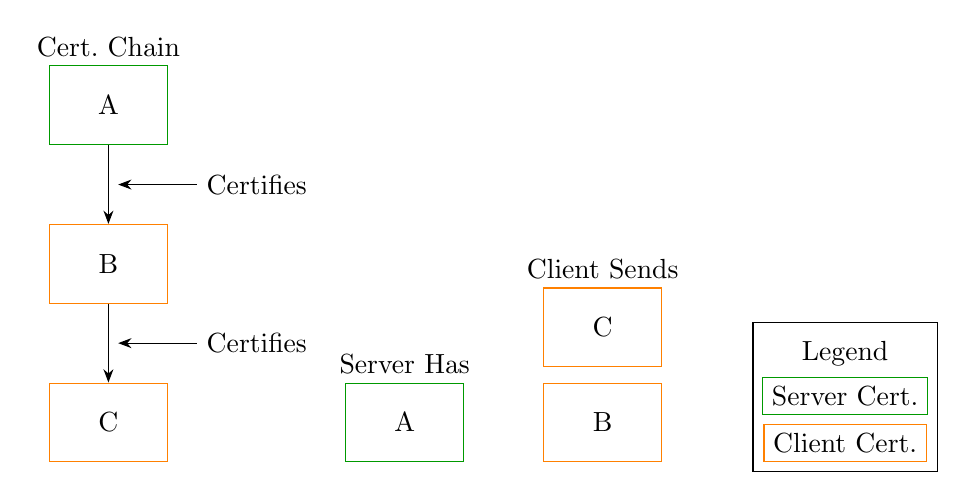
\begin{tikzpicture}
	% Styles.
	[s-cert/.style={rectangle,draw=green!60!black,minimum height=1cm,minimum width=1.5cm},
	c-cert/.style={rectangle,draw=orange,minimum height=1cm, minimum width=1.5cm}]
	% Certificate chain.
	\node (A) at (0, 0) [s-cert] {A};
	\node (B) [below=of A] [c-cert] {B};
	\node (C) [below=of B] [c-cert] {C};
	\draw[-Stealth] (A) -- (B)
		node[pos=0.5](a-cfies){};
	\node (a-cfies-txt) [right=of a-cfies] {Certifies};
	\draw[-Stealth] (a-cfies-txt) -- (a-cfies);
	\draw[-Stealth] (B) -- (C)
		node[pos=0.5](b-cfies){};
	\node (b-cfies-txt) [right=of b-cfies] {Certifies};
	\draw[-Stealth] (b-cfies-txt) -- (b-cfies);
	\node (txt) at (A) [above=0.5cm] {Cert.\ Chain};
	% Server certificates.
	\node (S-tmp) [right=of C] {};
	\node (S-A) [right=of S-tmp,s-cert] {A};
	\node (S-txt) at (S-A) [above=0.5cm] {Server Has};
	% Client certificates.
	\node (C-B) [right=of S-A,c-cert] {B};
	\node (C-C) at (C-B) [above=0.7cm,c-cert] {C};
	\node (C-txt) at (C-C) [above=0.5cm] {Client Sends};
	% Legend.
	\node (lanchor) at ($(current bounding box.south east) + (2, 0)$) {};
	\node (legend) at (lanchor) [above=1.1cm] {Legend};
	\node (l1) at (lanchor) [above=0.6cm,draw=green!60!black] {Server Cert.};
	\node (l2) at (lanchor) [above=0.0cm,draw=orange] {Client Cert.};
	\node [rectangle,draw,fit=(legend) (l1) (l2)] {};
\end{tikzpicture}
}
\end{makeimage}
\caption{Certificate chain where \texttt{A} is a trusted CA of the server and the client must send its certificate \texttt{C} followed by the intermediate certificate \texttt{B}.}
\end{figure}
\end{center}
After implementing a check for the entire peer certificate chain, my next problem was testing verification of the chain.  Consider the chain A -> B -> C, where A is trusted by the server and B and C are sent by the client.  I had been using OpenSSL's \texttt{s_client} command for testing, so the obvious approach was to place B and C into the file passed via the \texttt{-cert} argument; the first problem with this approach was that the certificates must be in a certain \emph{order}, specifically, the sender's certificate must come \emph{first}, followed by the certificate certifying the sender's certificate, and so on (see \htmladdnormallink{the RFC}{https://tools.ietf.org/html/rfc5246#section-7.4.2}).  In this case that meant sending C followed by B; specifying the certificates in the wrong order (B followed by C) was obvious, because \texttt{s_client} tried to use C's private key to verify B, which, of course, failed.  Putting them in the correct order, however, sent C while silently ignoring B.  After much gnashing of teeth, I decided to look into the source code, and, while combing through the parsing of the \texttt{-cert} option noticed an \emph{undocumented} (yes, not even in the \texttt{man} pages nor \texttt{-help} output) \texttt{-cert_chain} option.  After looking into it I ran the \texttt{s_client} command again with C sent via the \texttt{-cert} option and B sent via the \texttt{-cert_chain} option and was able to actually send a certificate chain to the server, and sanity was once again restored to my life.

\subsubsection{Testing}
Manually verifying changes is both a pain and error-prone, so I created a \htmladdnormallink{bash script}{https://github.com/clinew/inspircdtests/blob/master/ssl_strongcert.sh} in order to automatically test strong cert verification for InspIRCd on my system.  The tests check that the program runs without strong verification enabled, then turns verification on and checks that users can connect when their certificates use proper key type+sizes and algorithms, then checks that errors occur when invalid configuration options (such as non-existent algorithms) are specified, then finally checks that verification works correctly when the client passes a \emph{chain} of certificates.  It's not particularly exciting, but it gives peace of mind when rebasing on top of the latest stable release and when porting to newer versions of both OpenSSL and InspIRCd.

\subsection{Future Work}
After adding this feature I managed to find a series of functions that appeared as if they might do my heavy lifting for me.  The functions, found under the include directory as \texttt{ssl/ssl.h} were \texttt{SSL_set1_sigalgs_list()}, \texttt{SSL_set1_client_sigalgs_list()}, and a few similar variations.  Sadly, testing these show that they do not actually have the same functionality, although the signature algorithm list displayed after connecting via \texttt{s_client} was indeed different; presumably the signature algorithm is for session negation rather than peer certificate verification, but I am not yet sure as I have not yet Read The "Friendly" \strikeout{Manual} RFC.

The online man pages for the function also mentioned an \texttt{SSL_CONF} API, which might make option parsing easier; regardless, I didn't use it this time.


% Better Browsing With Firefox
\section{2018-01-17 Better Browsing With Firefox}
The Web is not what it once was, or at least not how I remember it.  It used to be like browsing a catalogue, with each link analogous to turning to a new page.  But the Web has transformed into something else entirely.  It is more like a \htmladdnormallink{two-way black mirror}{https://freedom-to-tinker.com/2017/11/15/no-boundaries-exfiltration-of-personal-data-by-session-replay-scripts} than a catalogue.  Every keystroke and mouse movement is logged and analyzed.  Users are tracked across unrelated websites by both visible widgets, invisible cookies, and more \htmladdnormallink{nefarious means}{https://en.wikipedia.org/wiki/Web_beacon}.  So-called "social media" sites analyze this data and censor their feeds in order to feed both themselves and their sponsors as much money as possible.  Basically, the Web has become a platform that consumes the user, rather than the user consuming the content of the Web.

Fortunately, there are ways to avoid being consumed by the Web and to create a more pleasant, catalogue-like browsing experience, but they are by no means obvious to the average person.  This blog will attempt to introduce the reader to some intermediate browsing techniques.  It assumes that the reader is already familiar with basic browser usage, and will then point out how, by installing a few add-ons, making a few configuration changes, and learning a few keystrokes, one's browsing experience can become both more controlled and more pleasant.  This requires work on the reader's part; it's not a give-me like most consumers desire, but tough shit, it's the world we currently live in.  This guide is divided into three sections, called "\htmladdnormallink{Power Levels}{https://www.youtube.com/watch?v=SiMHTK15Pik}", of increasing difficulty, with the first section requiring little to no work and having relatively little negative effect on one's browsing experience and a large positive effect, while the later sections require more work for often smaller gains.  Readers who are unsure of their skills should take a week or two in-between sections in order to familiarize themselves with any changes that they have made.

The Web browser of choice for this blog will be Firefox, because Firefox is \htmladdnormallink{Free Software}{https://www.gnu.org/philosophy/free-sw.en.html}.  Other common browsers, such as, but not limited to, Google Chrome, Safari, Microsoft Explorer, and Microsoft Edge are proprietary software and, therefore, \htmladdnormallink{considered harmful}{https://www.gnu.org/proprietary/proprietary.en.html}.  Make no mistake, Firefox has its flaws and its parent company, Mozilla Corporation, has made some \htmladdnormallink{questionable decisions}{http://lunduke.com/2017/12/17/mozilla-is-not-trustworthy}, but it's currently the best of the Free and featureful browsers to use.

\subsection{Power Level One}
\begin{figure}
\includegraphics[scale=0.5]{files/blog/2018_01_17_better_browsing_with_firefox/2018_01_17_ublockorigin_icon.png}
\caption{The uBlock Origin icon.}
\end{figure}
The first thing to do is to install the "uBlock Origin" add-on from the \htmladdnormallink{Mozilla Add-Ons}{https://addons.mozilla.org/en-US/firefox} webpage in order to block advertisements.  That's it.  Once it's installed, most advertisements will cease to be, and browsers without an ad-blocker will seem like a headache, because they are.  Sadly, a few sites will detect that one is using an ad-blocker and refuse to display any content, in which case you can disable the add-on \textit{for that site alone} by clicking on the uBlock Origin icon, then clicking the big ol' power-button icon in the drop-down menu that appears, but do note that most sites that are this ad-infested tend to suck and aren't worth reading anyways, in the same way that the trashiest magazines at the grocery checkout always have more advertisements than content in them.  Go figure.  Another icon worth noting is the little, Harry Potter-esque lightning icon, called the \textit{element zapper}.  Clicking on that icon will allow one to enter an element-zapper mode where one can select an element on the site for removal from their browser by clicking on it.  Hold \texttt{Shift} while clicking in order to continue removing elements, and press \texttt{Esc} to return to normal browsing mode.  Removals are not permanent, thus refreshing the page will reload any removed elements.  uBlock Origin can do this in part because it's actually a \textit{generic blocker} and not just an ad-blocker, but for now simply know that it's configured to block ads.

It's worth noting that there are other ad-blockers.  "AdBlock Plus" (ABP) is noteworthy for having been the de facto standard for a while before falling out of favor by many due to an \htmladdnormallink{"acceptable ads"}{https://adblockplus.org/acceptable-ads} campaign, in which certain, "unobtrusive" advertisements are not blocked by default and a portion of the revenue generated by the advertisements in sent to the ABP developers.  The AdBlock Plus add-on also tends to take up far more memory than uBlock Origin, which gave me issues on my low-memory machines, thus I prefer uBlock Origin for that reason alone.  There's also "uBlock", which was originally developed by the author of uBlock Origin, but apparently there were some issues and now the original author is working on uBlock Origin and that's what I've decided to use.  Feel free to check out the other one if you are so inclined.

\begin{figure}
\includegraphics[scale=0.5]{files/blog/2018_01_17_better_browsing_with_firefox/2018_01_17_httpseverywhere_icon.png}
\caption{The HTTPS Everywhere icon.}
\end{figure}
The next thing to do is to install the "HTTPS Everywhere" add-on developed by the \htmladdnormallink{Electronic Frontier Foundation}{https://www.eff.org/} (EFF).  A brief explanation is in order: HyperText Transfer Protocol (HTTP) is the protocol used for the Web, and HTTP\textbf{S} is, roughly speaking, the \textit{\textbf{S}ecure} version of that protocol.  HTTPS is useful because it's the reason \htmladdnormallink{crackers}{https://stallman.org/articles/on-hacking.html} cannot easily break into your bank account or use your credit card when you are browsing the web.  Many sites offer both secured and unsecured versions of their webpages but configure their websites such that users must explicitly request the secure version of the website by prefixing the address with \texttt{https://}, which is a giant pain in the ass.  HTTPS Everywhere fixes this problem by automatically \textit{rewriting} (a.k.a. "changing") any HTTP addresses to their secure, HTTPS variants, no user intervention required.  This is done through a database of sites that comes with the program; the database knows how to rewrite addresses for different sites.  Although a few, very obscure sites may not have their addresses rewritten, the vast majority will.

Lastly, it is worth learning one mouse click technique and a few simple key-commands.  Most mice have a scroll wheel in the middle, and that scroll wheel can be pressed in order to generate a "middle-mouse button click", or "middle-click" for short.  Middle-clicking a link will open said link in a new tab.  This is far faster than going through the tedious process of right-clicking the link and then selecting "Open in New Tab" from the drop-down menu.  It's a serious time-saver.  Use it.  The middle-mouse click can also be used to close a tab by clicking on the tab itself.  Ever accidentally close a tab and then realized that it shouldn't have been closed?  Type \texttt{Ctrl-Shift-T} to bring it back!  Continue typing the command in order to bring back tabs in the order in which they were closed.  Finally, \texttt{Ctrl-F} can be used to \textit{Find} text within a webpage.  Just in case one wasn't aware.

That's it for this first section.  One's browsing experience should now be ad-free, far more secure, and hopefully a little bit smoother with those middle-clicks.  There probably won't be any disruption in one's browsing experience, but take some time to get used to it before proceeding onto the next section.

\subsection{Power Level Two}
This section will impact one's browsing experience far more than the previous section.  This section also plays the largest part in disabling the two-way mirror "functionality" of the Web.  This involves changing a few configuration options, installing a new add-on, and finally learning a few keyboard shortcuts.

Begin by making some configuration changes to Firefox that will cause each \textit{session} to be independent of the others.  In other words, each time Firefox is closed and opened it will be as if no websites had been visited during the previous time Firefox was open, even if they were, as if Firefox had just been installed, except, of course, the add-ons, bookmarks, and other user-defined settings will remain.  I could try and describe the bloody icons that lead to the \texttt{Preferences} menu, but it'll be easier if I tell you to simply type \texttt{F10} to open the old-style text-based menu and then navigate to \texttt{Edit -> Preferences}.  From there, click on the tab labeled \texttt{Privacy}, then find the section labelled \texttt{History} and change the corresponding drop-down to \texttt{Never remember history}.  Likewise, next find the section labelled \texttt{Location Bar} and uncheck all of the boxes.  Lastly, click on the tab labelled \texttt{Advanced}, then another tab labelled \texttt{Network} and finally the section labelled \texttt{Cached Web Content} and check the \texttt{Override automatic cache management} checkbox and then set the specified value to \texttt{0 MB}.  That should make each browsing session far more independent and thus make tracking more difficult, but it will be noticeable as many sites that require a login will no longer "remember" one's username and one will thus have to type it in again.

\begin{figure}
\includegraphics[scale=0.5]{files/blog/2018_01_17_better_browsing_with_firefox/2018_01_17_noscript_icon.png}
\caption{The NoScript icon.}
\end{figure}
Next comes the biggest change: installing the "NoScript" add-on.  This add-on is what allows one to selectively enable and disable JavaScript.  Unlike plain HTML, JavaScript is actually code that is sent by the web server and run on the user's computer.  This code is what allows the browser to track the user's mouse movements, keystrokes, and gather various information about the user's system.  The fact that browsers run arbitrary JavaScript code on the user's computer is a large part of what turns the Web from a catalogue into a two-way mirror (confusingly enough, JavaScript has no relationship to the Java programming language).  What NoScript does is to give one some control over what JavaScript is run on their computer.  The default is to block all JavaScript, which will cause many sites to break, but scripts can be allowed on a per-site basis by clicking the NoScript icon and then selecting \texttt{Temporarily allow from <address>} from the drop-down menu where \texttt{<address>} is the name of the site that the JavaScript is loaded from, and when the drop-down menu is closed the site will automatically reload with the selected scripts enabled.  Note that most sites load JavaScript from multiple sources, thus the \texttt{Temporarily allow all this page} option can come in handy when one wants to load all scripts on the site, but note, however, that some scripts will then drag in other scripts, and thus for certain sites one will have to "allow all" for the site multiple times.  Note that any allowances made will apply to \textit{all} tabs that one has opened, not just the current tab.  When one no longer wishes to allow scripts, clicking the icon again and selecting the \texttt{Revoke temporary permissions} will disable all scripts and refresh the sites whose scripts were revoked.  It's actually quite simple once one gets the hang of it.

After using NoScript for a while one will inevitably notice that certain addresses come up again and again.  Most notorious in my opinion is \texttt{google-analytics.com}.  Since I have absolutely no desire to be analyzed by The Googlaug ever, I banished the script permanently by clicking the NoScript icon, then selecting \texttt{Untrusted -> Mark google-analytics.com as untrusted}, thus removing it from the drop-down menu.  Good riddance.  The drop-down menu can be customized by selecting \texttt{Options} and then the \texttt{Appearance} tab and toggling the various boxes.  It can be useful to uncheck the \texttt{Allow [...]} and \texttt{Allow all this page} boxes if one does not wish to even accidentally give some scripts permanent permission.

Now, NoScript actually does a little more than just block JavaScript, it also protects against a few types of Web-based attacks by blocking \htmladdnormallink{Cross-Site Scripting (XSS)}{https://en.wikipedia.org/wiki/Cross-site_scripting} and implementing \htmladdnormallink{Application Boundary Enforcer (ABE)}{https://noscript.net/abe/}.  Although these are generally considered a Good Thing (TM), they occasionally cause problems with crappy Web portals, for example, at one's local library where one is required to agree to a Terms of Service (ToS), and need to be disabled.  ABE can usually be worked around by choosing the "Unsafe Reload" option after it has been triggered, but both can be disabled by opening the options window, selecting the \texttt{Advanced} tab and then selecting either the \texttt{XSS} or \texttt{ABE} tab and turning the offending feature off.  With that one should now have some basic control over the JavaScript run on one's own computer.

A few more useful key-commands are now in order.  First, \texttt{Ctrl-L} and \texttt{Ctrl-J} move the cursor to the Location and Search Bar, respectively.  For tab-management, \texttt{Ctrl-T} opens a new tab, \texttt{Ctrl-W} closes the current tab, and \texttt{Ctrl-Q} quits the browser program; because the \texttt{Q} key is right next to the \texttt{W} key, it's a good idea to keep the "Warn me when I attempt to close multiple tabs" checkbox enabled.  Lastly, use \texttt{Ctrl-PgUp} (Page Up) and \texttt{Ctrl-PgDn} (Page Down) in order to move to the previous and subsequent tab, respectively.

Thus ends the second section.  Each browser session should now be more independent and two-way mirror functionality will be disabled by default.  These are both rather large changes to make, but they offer significant privacy and security advantages, so the added difficulty is often worthwhile.  Make sure to become comfortable with these changes before moving onto the next section.

\subsection{Power Level Three}
As explained in the first section, uBlock Origin is actually a \textit{generic blocker}, meaning that it can block more than just ads.  Ad-blocking is actually done via a \textit{filter list} which is provided by a third party, and there exist more than just ad-filter lists, for example, filter lists to block embedded tracking widgets from sites like Farcebook.  In order to view the filter lists, click on the uBlock Origin icon and then click on the icon that looks like, uh, well, three lines with some kind of slider-thingies on it (damn icons) in order to open the "dashboard", and then click on the "3rd party filters" tab in order to view a default list of filters.  Learn more about each filter by clicking on the house icon in order to be directed to a webpage containing information about the filter, and enable/disable filters by checking/unchecking their respective boxes.  I like "Fanboy's Social Blocking List" myself.  One can also manually update their lists by clicking the obvious "Update Now" button while on this tab.

Filter lists are nice for most uses, but sometimes one needs custom filters on a site; this can be done by clicking "I am an advanced user" in the dashboard's "Settings" tab and thus enabling \textit{dynamic filtering}; make sure to read the corresponding documentation under \htmladdnormallink{required reading}{https://github.com/gorhill/uBlock/wiki/Advanced-user-features} before trying to apply any dynamic filters; they are not covered here because the existing documentation is better than what I would write.  Note that after enabling dynamic filtering it's interesting enough to simply click on the uBlock Origin icon after loading a site and seeing which sites one's browser has connected to.  In a similar vein to the zapper icon (in the menu that appears after clicking the uBlock Origin icon), the eye-dropper, or \textit{element picker}, helps create custom filter rules rather than simply removing an element until the page is reloaded, but be careful about the filters it creates unless one wants to filter more than intended.  Adding custom filters in more of an art than a science, but it provides incredible control over which services get to track one's virtual movement across the Web.

When customizing Firefox, one might be tempted to naively believe that, after clicking on the gear icon and perusing all sections and tabs and setting things up as one desires that they're finished with all possible non-add-on-based customizations.  However, Firefox, in fact, actually has a, well, it's not exactly \textbf{hidden}, but \textbf{unadvertised}, perhaps, customization menu that can be reached by typing \texttt{about:config} into the address bar (then hitting \texttt{Enter}, obviously).  This page consists of a list of \textit{preferences} with a \textit{type} and \textit{value} and whose values can be customized by the user.  A full discussion of all preferences in this menu would likely require an entire encyclopedia, so only a few noteworthy preferences are mentioned here.  First off is the \texttt{UserAgent}, which is a string containing various client metadata such as operating system, browser vendor, browser version, \&c, and which is sent to the web server when the connection is first established so that the web server can serve up client-specific \htmladdnormallink{hacks}{https://en.wikipedia.org/wiki/Hack_(computer_science)}, \htmladdnormallink{nevermind that the whole damn point of the web was to be platform-independent}{http://www.catb.org/~esr/html-hell.html}.  One can view their \texttt{UserAgent} by navigating to \texttt{about:} in the address bar, and one can customize it in the \texttt{about:config} menu by right-clicking then selecting \texttt{New -> String} and then giving the preference name \texttt{general.useragent.override} and then providing whatever value one wants; check \texttt{about:config} to confirm.  Note that poorly-designed sites will break if they can't supply custom browser-specific hacks, for example, this is what Googlaug Voice looks like with the classy \texttt{UserAgent} of "Fuck JavaScript":
\begin{figure}
\includegraphics[scale=0.33]{files/blog/2018_01_17_better_browsing_with_firefox/2018_01_17_googlaug_voice.png}
\caption{These modern interfaces really know how to cut down on bloat!}
\end{figure}
Note that using a custom \texttt{UserAgent} is \htmladdnormallink{probably less anonymous than one might think}{https://panopticlick.eff.org/}.

A few other noteworthy preferences are \texttt{javascript.options.asmjs} which allows JavaScript to run native code on one's computer and will probably cause some security nightmare within the next decade or two (set it to \texttt{false} now).  One may also wish to set \texttt{webgl.disabled} to \texttt{true}, although NoScript already forbids WebGL by default.  Due to \htmladdnormallink{recent events}{https://sircmpwn.github.io/2017/12/16/Firefox-is-on-a-slippery-slope.html} one will probably want to set \texttt{experiments.enabled} to \texttt{false}.  Note that while one might be tempted to set \texttt{javascript.enabled} to \texttt{false}, JavaScript is actually used internally by the browser and add-ons, and thus disabling it here actually causes add-ons to not function properly, relying on NoScript is recommended instead.

This section has been rather open-ended, because customizations at this point have become, well, highly-customized.  Nonetheless, one should now have an idea of how to go about blocking content on websites they visit and performing deep configuration of Firefox.

\subsection{Conclusion}
That's it for this guide.  Hopefully one's browser experience is now both cleaner and more controlled than it had been before.  While it may have been a large amount of information to take in, please understand that there is still much more to be learned about the Web and its oftentimes questionable behaviour, and please note that none of these techniques are meant to make one anonymous, as that is the aim of other projects such as \htmladdnormallink{Tor}{https://torproject.org} and \htmladdnormallink{TAILS}{https://tails.boum.org}.  Regardless, one who has followed this guide should now be able to begin taking back control of their Web experience.  Good luck.


% 4.9-4.14 Kernel Upgrade USB Woes
\section{2018-01-08 4.9-4.14 Kernel Upgrade USB Woes}
Given the recent concerns over the Meltdown/Spectre vulnerabilities and the release of \htmladdnormallink{new stable kernels}{https://lwn.net/Articles/743246/}, I figured that now would be a good time to do a quick kernel upgrade.  As you have probably surmised by the very existence of this blog post, the "quick" upgrade turned into a bit of a headache.

Rather than using another 4.9 kernel with a backported mitigation, I decided that now would be a good time to upgrade to the newer 4.14 kernel.  The usual process went smoothly: downloading, verifying the signature, updating the configuration, compiling, and finally booting.  Except there was one little problem after booting: I couldn't enter my passphrase from my keyboard in order to decrypt the root filesystem.  Huh?  The keyboard, which is a USB keyboard, had worked before the BIOS hand-off, and it still had power, but no key-presses, even SysRq keys, had any effect.  Other than that, the kernel seemed perfectly fine, no backtraces or nasty error messages being spewed out.

Okay, well, at this point I was rather dumbfounded.  Nothing in the output of \texttt{make oldconfig} that I could recall suggested something that would break my USB keyboard, and the only thing that I really cared about in this upgrade was the new Kernel Page-Table Isolation (KPTI) feature, but maybe this was some weird bug with it and my \texttt{initramfs}, so I tried disabling it, recompiling the kernel, and booting the recompiled kernel.  Still broken.  So, at least the security feature that I'd upgraded for wasn't the source of my woes, but that didn't solve my problem.  At this point it also occurred to me that no messages for the attached USB storage device were showing up, either, so this was some kind of USB problem.  Perhaps the problem was specific to the front ports?  I decided to try the back ports, which are attached directly to the motherboard, and did not have any luck there, either.

Perhaps I'd missed something when updating the configuration, so I saved my new configuration and re-ran \texttt{make oldconfig} on a copy of the old configuration and noted any options that \textit{might possibly} be affecting my USB devices.  A few possibilities emerged, including \texttt{X86_MCELOG_LEGACY} (the \texttt{initramfs} is rather old), \texttt{SERIAL_DEV_BUS} (are the USB devices connected to the motherboard via serial?), \texttt{RC_CORE} (uhh do I have video capture?), \texttt{USB_PCI}, and \texttt{USB_HUB_USB251XB}.  The latter two options seemed the most suspicious.  The help information for \texttt{USB_PCI} reads:
\begin{quote}
\begin{verbatim}
	A lot of embeded system SOC (e.g. freescale T2080) have both
	PCI and USB modules. But USB module is controlled by registers
	directly, it have no relationship with PCI module.

	When say N here it will not build PCI related code in USB driver.
\end{verbatim}
\end{quote}
English is obviously not their native language, but code isn't mine, so fair's fair.  It sounds like there's PCI code in the USB module for\ldots~no reason?  Well, I don't have any USB hubs connected via PCI add-on cards, so this should be safe left disabled.  Regarding \texttt{USB_HUB_USB251XB}, perhaps some hub-specific code got moved into a separate option and I happen to be using that hub.

No clear winner emerged, so I opened the case in order to examine how the USB ports were connected and what hubs were in use:
\begin{figure}
\includegraphics[scale=0.5]{files/blog/2018_01_08_kernel_upgrade_usb_woes/motherboard.png}
\caption{"Can you find the PCI USB on this motherboard?  Neither could we."}
\end{figure}
The back ports are directly connected to the motherboard, and the front ports are connected by some\ldots~thing to the motherboard.  I have no idea how components on the motherboard are interconnected (I2C?, serial?, gnomes?), but the USB hubs are certainly not connected via PCI cards, and I couldn't find any "USB251XB" markings on or around the hubs, not that I could particularly make out the small, cryptic writings on the board anyhow.  After blowing out some dust and a couple of sneezes later I went back to scratching my head.  Perhaps \texttt{make oldconfig} didn't tell me everything.  I decided to run a \texttt{diff -u} in-between the old and new configuration, and one line in particular caught my eye:
\begin{quote}
\begin{verbatim}
	-CONFIG_USB_UHCI_HCD=y
\end{verbatim}
\end{quote}
Now I cannot for the life of me remember what each of the \texttt{_HCI} USB configurations refer to what vendor/version combination, but this seemed like a \textit{very} strange omission.  Going into \texttt{menuconfig} and searching for the option was even more telling:
\begin{quote}
\begin{verbatim}
	Prompt: UHCI HCD (most Intel and VIA) support
\end{verbatim}
\end{quote}
"most Intel", eh?  So why was this option magically unselected?
\begin{quote}
\begin{verbatim}
	Depends on: USB_SUPPORT [=y] && USB [=y] && (USB_PCI [=n] || USB_UHCI_SUPPORT_NON_PCI_HC [=n])
\end{verbatim}
\end{quote}
Right, so, disabling the new \texttt{USB_PCI} option will \textit{silently} disable \texttt{USB_UHCI_HCD} \textit{even if it was already selected}.  Could this be my problem?  I enabled both \texttt{USB_PCI} and \texttt{USB_UHCI_HCD}, recompiled, booted, and, lo and behold, my USB devices started working again.

So much for a "quick" upgrade.  While I'm glad to have things working again, it would have been nice if the \texttt{USB_PCI} help had clarified that whether or not PCI code is needed in the USB module \textit{depends on the system}, because the current wording suggests that it \textit{never} has any relationship to the PCI module ("it have no relationship with PCI module", said without qualifications).  Something along the lines of, "in these embedded systems, the USB module has no relationship to the PCI module" would have been better.  It also would have been nice if the \texttt{USB_UHCI_HCD} options wasn't silently disabled, but that may be a limitation of the Kconfig language; I don't know.  At least things are working again\ldots~at least until the other cache vulnerabilities start being exploited \texttt{;)}.


% Booting BeagleBone Black With an Initramfs
\section{2017-10-05 Booting BeagleBone Black With an Initramfs}
\begin{center}
\begin{figure}
\begin{makeimage}
\newcommand{\fn}[1]{\hspace*{1ex}\texttt{#1}}
\fbox{
\begin{tabular}{l l}
Before: & After: \\
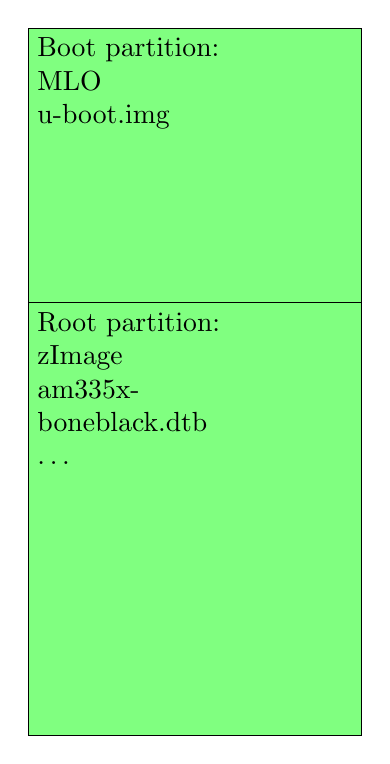
\begin{tikzpicture}
	\node at (0, 0) [rectangle split,rectangle split parts=2,rectangle split part fill={green!50, green!50},align=left,draw,text width=4cm]
		{\rule[-3cm]{0cm}{3cm}\parbox[t]{3cm}{Boot partition: \\ \fn{MLO} \\ \fn{u-boot.img}}
		\nodepart{two} \rule[-5cm]{0cm}{5cm}\parbox[t]{3cm}{Root partition: \\ \fn{zImage} \\ \fn{am335x-boneblack.dtb} \\ \fn{\ldots}}};
\end{tikzpicture}
&
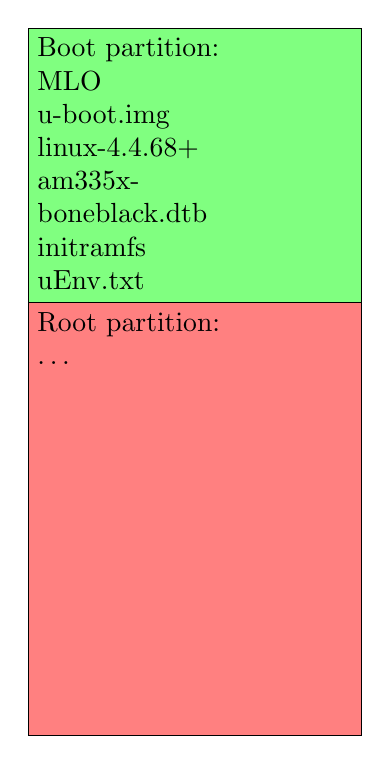
\begin{tikzpicture}
	\node at (0, 0) [rectangle split,rectangle split parts=2,rectangle split part fill={green!50, red!50},align=left,draw,text width=4cm]
		{\rule[-3cm]{0cm}{3cm}\parbox[t]{3cm}{Boot partition: \\ \fn{MLO} \\ \fn{u-boot.img} \\ \fn{linux-4.4.68+} \\ \fn{am335x-boneblack.dtb} \\ \fn{initramfs} \\ \fn{uEnv.txt}}
		\nodepart{two} \rule[-5cm]{0cm}{5cm}\parbox[t]{3cm}{Root partition: \\ \fn{\ldots}}};
\end{tikzpicture}
\end{tabular}
\begin{tabular}{c l}
\multicolumn{2}{c}{\textbf{Legend}} \\

\begin{tikzpicture}
	\node at (0, 0) [fill=green!50,draw] {};
\end{tikzpicture} & Unencrypted \\

\begin{tikzpicture}
	\node at (0, 0) [fill=red!50,draw] {};
\end{tikzpicture} & Encrypted
\end{tabular}
}
\end{makeimage}
\caption{Visualization of the SD Card before and after modifications.  Contents are not to scale.}
\end{figure}
\end{center}

The instructions for installing Gentoo on my BeagleBone Black (BBB)\htmladdnormallink{[1]}{https://wiki.gentoo.org/wiki/BeagleBone_Black} gave me a working OS, but one without the root partition encrypted.  Unencrypted OSes make me sad, but an encrypted root partition means using an \texttt{initramfs}; to make matters more complicated, the kernel and device tree are on the root partition, but they need to be on the boot partition (because the root partition will be encrypted).  This blog will explain how I was able to make these changes; it will not cover creating an \texttt{initramfs} nor creating an encrypted root partition using LUKS and \texttt{cryptsetup}.

\subsection{Das U-Boot}
Das U-Boot, colloquially known simply as "U-Boot", is roughly analogous to the BIOS and/or UEFI portion of normal desktop towers.  Like desktops, the boot process can be interrupted and the user taken to a configuration interface by typing a certain key early on in the boot process.  For the BBB, this can be done by pressing the 'Space' button, which takes the user to a Command-Line Interface (CLI); from here, \texttt{help} may be run in order to provide a list of commands or to print usage information for a specific command.  One of the most useful commands to run is \texttt{printenv}, which will list all of the environment variables; these variable are important because their values can be either simple values or an entire script.  It is these variables that must be modified in order to load and boot an \texttt{initramfs}, kernel, and device tree file from the boot partition.

While one can modify the environment variables before each boot, this is extremely tedious.  Thankfully, U-Boot allows one to define a \texttt{uEnv.txt} file in the boot partition that will be read in before the boot process is completed and which will set the environment variables as specified in the file.  Thus one can simply write this file rather than constantly modify the environment variables at each boot.

\subsection{uEnv.txt}
This section will explain what variables I added/modified and why I modified them.  Though they are all crammed together in the actual file, for conceptual purposes I will divide them into three categories: filename definitions, load scripts, and boot scripts.

The first of the sections, filename definitions, is straightforward enough:
\begin{quote}
\begin{verbatim}
	# BEFORE
	bootfile=zImage
	# AFTER
	bootfile=linux-4.4.68+
	rdfile=initramfs
\end{verbatim}
\end{quote}
Although changing the name from \texttt{zImage} to \texttt{linux-4.4.68+} isn't strictly necessary, I prefer to have my kernels include their version in the name as it makes booting, upgrading, and dealing with regressions easier.  The \texttt{rdfile} variable is added for consistency with the existence of the \texttt{bootfile} variable, and is used later.  Note that the same \texttt{initramfs} can often be used across multiple kernel versions.

The second section, load scripts, consists of the series of commands used to load the kernel, initramfs, and device tree into memory:
\begin{quote}
\begin{verbatim}
	# BEFORE
	loadimage=load ${devtype} ${bootpart} ${loadaddr} ${bootdir}/${bootfile}
	loadfdt=load ${devtype} ${bootpart} ${fdtaddr} ${bootdir}/${fdtfile}
	loadramdisk=load mmc ${mmcdev} ${rdaddr} ramdisk.gz
	# AFTER
	loadimage=fatload mmc ${mmcdev} ${loadaddr} ${bootfile}
	loadfdt=fatload mmc ${mmcdev} ${fdtaddr} ${fdtfile}
	loadramdisk=fatload mmc ${mmcdev} ${rdaddr} ${rdfile}
\end{verbatim}
\end{quote}
A few things are worth noting here.  First is that I ignored the \texttt{devtype} and \texttt{bootpart} variables and just loaded the kernel (\texttt{loadimage}), device tree (\texttt{loadfdt}), and initramfs (\texttt{loadramdisk}) directly from the MMC (SD Card), since that is what I wanted; this worked on my SD Card, but may be fragile on other configurations, use at your own risk!  Second, there is already an instruction for loading a ramdisk which, from a cursory glance of other environment variables, appears to be associated with boot code for a live OS rather than an \texttt{initramfs} for booting; since I currently am not interested in nor know how to use this functionality, it appears safe to modify.  Last, I removed the \texttt{bootdir} prefix for the kernel and device tree filepaths, since I'm simply going to place them at the root directory of the boot partition.

The last section, boot scripts, is the most complicated section, because it contains the commands and logic needed to actually boot the system:
\begin{quote}
\begin{verbatim}
	# BEFORE
	args_mmc=run finduuid;setenv bootargs console=${console} ${optargs} root=PARTUUID=${uuid} rw rootfstype=${mmcrootfstype}
	mmcloados=run args_mmc; if test ${boot_fdt} = yes || test ${boot_fdt} = try; then if run loadfdt; then bootz ${loadaddr} - ${fdtaddr}; else if test ${boot_fdt} = try; then bootz; else echo WARN: Cannot load the DT; fi; fi; else bootz; fi;
	# AFTER
	args_mmc=run finduuid;setenv bootargs console=${console} ${optargs} root=/dev/mapper/mmcblk0p2 initrd=initramfs rw rootfstype=${mmcrootfstype}
	mmcloados=run args_mmc; run loadramdisk; if test ${boot_fdt} = yes || test ${boot_fdt} = try; then if run loadfdt; then bootz ${loadaddr} ${rdaddr} ${fdtaddr}; else if test ${boot_fdt} = try; then bootz; else echo WARN: Cannot load the DT; fi; fi; else bootz; fi;
\end{verbatim}
\end{quote}
While the commands may appear relatively complex, the modifications are actually pretty simple.  For \texttt{args_mmc}, the \texttt{root=PARTUUID=\${uuid}} had to be changed to the mapping set up by the encryption scripts, in my case to \texttt{root=/dev/mapper/mmcblk0p2}; the argument \texttt{initrd=initramfs} was also added to let the kernel know about the \texttt{initramfs} file (but may not strictly be necessary in this context).  Two modifications were made to \texttt{mmcloados}: the first was to load the initramfs by calling \texttt{run loadramdisk;}, the second was to change the \texttt{bootz} command to contain the address of the \texttt{initramfs} to load (\texttt{rdaddr}) rather than not loading one (\texttt{-}).

Thus with each of these modifications I was able to boot with an encrypted root partition.  Hopefully you will have the same luck, and don't forget to copy your files from the root partition to the boot partition!


% Adding Certificate Revocation Lists (CRLs) to an Existing OpenSSL Implementation.
\section{2017-09-22 Adding Certificate Revocation Lists (CRLs) to an Existing OpenSSL Implementation}
I recently took it upon myself to add Certificate Revocation List (CRL) functionality to an SSL-enabled program (\htmladdnormallink{InspIRCd}{https://github.com/inspircd/inspircd/pull/1370}).  This blog details both the code that I used and some unexpected functionality regarding how CRLs behave.  Hopefully this blog will prove useful to someone else who needs to tread this path.

\subsection{Code Itself}
The code itself is actually quite simple, consisting of two basic steps: loading the CRL files and then enabling CRL checking.  In order to load the CRL files, begin by getting the \texttt{X509_STORE *} from the \texttt{SSL_CTX *} by calling \texttt{SSL_CTX_get_cert_store(3)}, then load the CRL files into the \texttt{X509_STORE *} by calling \texttt{X509_STORE_load_locations()} with the specified CRL file and path locations.  The definition of the functions can be found in \texttt{openssl/x509_vfy.h} in your system's include file directory.  The code looks something like:
\begin{quote}
\begin{verbatim}
	SSL_CTX *ctx = sslctx; // Defined elsewhere.
	X509_STORE *store;
	char *crlfile = "/path/to/single/file.pem";
	char *crlpath = "/path/to/entire/directory";

	if (!(store = SSL_CTX_get_cert_store(ctx))) {
		fprintf(stderr, "No cert store found\n");
		return -1;
	}
	if (!X509_STORE_load_locations(store, crlfile, crlpath)) {
		fprintf(stderr, "Unable to load CRL files\n");
		return -1;
	}
\end{verbatim}
\end{quote}
This will load the CRL files, but will not enable CRL checking; this has to be done by setting a flag value in the \texttt{X509_STORE *}.  There at least two possible options: one is to check only the leaf certificate, the other is to check all certificates in the chain.  The former option can be accomplished by setting only \texttt{X509_V_FLAG_CRL_CHECK} while the latter can be accomplished by setting two flags \texttt{X509_V_FLAG_CRL_CHECK | X509_V_FLAG_CRL_CHECK_ALL}.  The latter option (the entire chain) is almost certainly what you want.
\begin{quote}
\begin{verbatim}
	char* crlmode; // Defined elsewhere.
	int crlflags;

	if (!strcmp(crlmode, "chain")) {
		crlflags = X509_V_FLAG_CRL_CHECK | X509_V_FLAG_CRL_CHECK_ALL;
	} else if (!strcmp(crlmode, "leaf")) {
		crlflags = X509_V_FLAG_CRL_CHECK;
	} else {
		fprintf(stderr, "Unknown flag mode '%s'\n", crlmode);
		return -1;
	}
	if (X509_STORE_set_flags(store, crlflags) != 1) {
		fprintf(stderr, "Unable to set flags\n");
		return -1;
	}
\end{verbatim}
\end{quote}
\ldots and that's it!  CRLs should now be enabled for your program.  However, do not rest easily just yet, as CRLs offer several pitfalls for the unwary, as detailed below.

\subsection{Missing CRL Files}
Consider the following, simple certificate chain:
\begin{center}
\begin{figure}
\begin{makeimage}
\fbox{
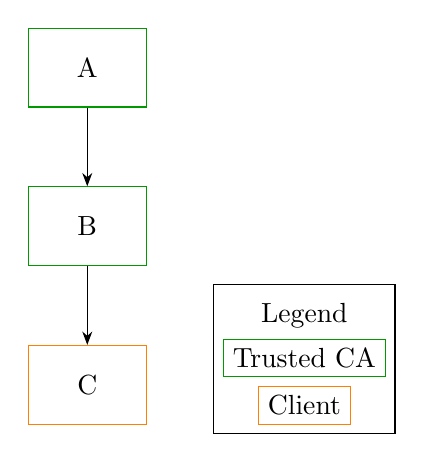
\begin{tikzpicture}
	% Styles.
	[ca/.style={rectangle,draw=green!60!black,minimum height=1cm,minimum width=1.5cm},
	leaf/.style={rectangle,draw=orange,minimum height=1cm, minimum width=1.5cm}]
	% Certificates.
	\node (A) at (0, 0) [ca] {A};
	\node (B) [below=of A] [ca] {B};
	\node (C) [below=of B] [leaf] {C};
	\draw[-Stealth] (A) -- (B);
	\draw[-Stealth] (B) -- (C);
	% Legend.
	\node (lanchor) at ($(current bounding box.south east) + (2, 0)$) {};
	\node (legend) at (lanchor) [above=1.1cm] {Legend};
	\node (l1) at (lanchor) [above=0.6cm,draw=green!60!black] {Trusted CA};
	\node (l2) at (lanchor) [above=0.0cm,draw=orange] {Client};
	\node [rectangle,draw,fit=(legend) (l1) (l2)] {};
\end{tikzpicture}
}
\end{makeimage}
\caption{Simple certificate chain, where A and B are CAs and C is the client.}
\end{figure}
\end{center}
The server trusts Certificate Authorities (CAs) A and B to issue valid certificates, thus C's certificate will be accepted.  Without CRLs this scenario will work as expected, C will be able to connect to the server without a problem.  Now, assume that the server enables CRLs, generates a CRL for A, and then configures itself to use A's CRL; a CRL for B is not generated as B has not revoked any certificate and thus there doesn't \emph{seem} to be any need to generate a CRL for B.  As you can probably guess by now, C will not be able to connect in this scenario, because the default CRL-checking method requires \emph{every} CA in the chain to have a CRL file loaded, thus C cannot connect unless both A \emph{and} B generate CRL files, \emph{even if they have no revoked certificates}.
\begin{center}
\begin{figure}
\begin{makeimage}
\fbox{
\begin{tikzpicture}
	% Styles.
	[ca/.style={rectangle,draw=green!60!black,minimum height=1cm,minimum width=1.5cm},
	leaf/.style={rectangle,draw=red,minimum height=1cm, minimum width=1.5cm},
	x/.pic={
		\draw[--] (-1mm,1mm) -- (1mm,-1mm);
		\draw[--] (-1mm,-1mm) -- (1mm,1mm);
	}]
	% Certificates.
	\node (A) at (0, 0) [ca] {A};
	\node (B) [below=of A] [ca] {B};
	\node (C) [below=of B] [leaf] {C};
	\draw[-Stealth] (A) -- (B);
	\draw[-Stealth] (B) -- (C)
		node[pos=0.5](fail){}
		pic [pos=0.5,red] {x};
	\node (error) [right=of fail] {No CRL file for B};
	\draw[-Stealth] (error) -- (fail);
	% Legend.
	\node (lanchor) at ($(current bounding box.south east) + (1.5, 0)$) {};
	\node (legend) at (lanchor) [above=1.1cm] {Legend};
	\node (l1) at (lanchor) [above=0.6cm,draw=green!60!black] {Trusted CA};
	\node (l2) at (lanchor) [above=0.0cm,draw=red] {Client};
	\node [rectangle,draw,fit=(legend) (l1) (l2)] {};
\end{tikzpicture}
}
\end{makeimage}
\caption{Each CA is required to have a CRL file.}
\end{figure}
\end{center}

The consequence of this is that enabling CRL-checking requires gathering CRL files, a task that is likely non-trivial.  The alternative is to override OpenSSL's verify callback by defining your own verify function and then telling OpenSSL to use said function with \texttt{X509_STORE_set_verify_cb(3)}.  I, however, do not intend to touch that with a 10-foot pole.

\subsection{Using a CRL Path}
Suppose that you wish to use a directory to store CRL files separately for each CA (instead of one big CRL file), then have OpenSSL load in each CRL file from this directory.  An obvious benefit of this approach is that it allows you to create a separate CRL file for each CA; using the certificate chain from the previous section, this would mean a directory containing both \texttt{crl/a.pem} and \texttt{crl/b.pem}.  One would think that it would be enough to place each CRL file in said directory, then point OpenSSL to said directory, but that actually doesn't work.

While OpenSSL indeed expects each CA to have its own CRL file, it expects the CA file to be named in a very specific manner; it expects the file to be named as the concatenation of the first part of the \emph{hash} of its issuer name and \texttt{.rX} where \texttt{X} starts as \texttt{0} and is incremented for each hash collision that occurs.  For example, suppose the hash of CA B is \texttt{deadbeef}, then its CRL filename is expected to be \texttt{deadbeef.r0}.  Arguably, the easiest way to support this hash-based filename is to create the actual CRL file with the name of its respective issuer, then create the symbolic link for OpenSSL, which can be done by something like:
\begin{quote}
\begin{verbatim}
	for crl in `ls *.pem`; do
		hash=$(openssl crl -hash -in "${crl}" -noout)
		# Just assume no collisions for simplicity.
		ln -s "${crl}" "${hash%$'\n'}.r0"
	done
\end{verbatim}
\end{quote}
\ldots which generates a hash for each file suffixed with \texttt{.pem} in the current directory (WARNING: does not take into account hash collisions).  With the symbolic links created, you should now be able to use a CRL path.

\begin{center}
\begin{figure}
\begin{makeimage}
\fbox{
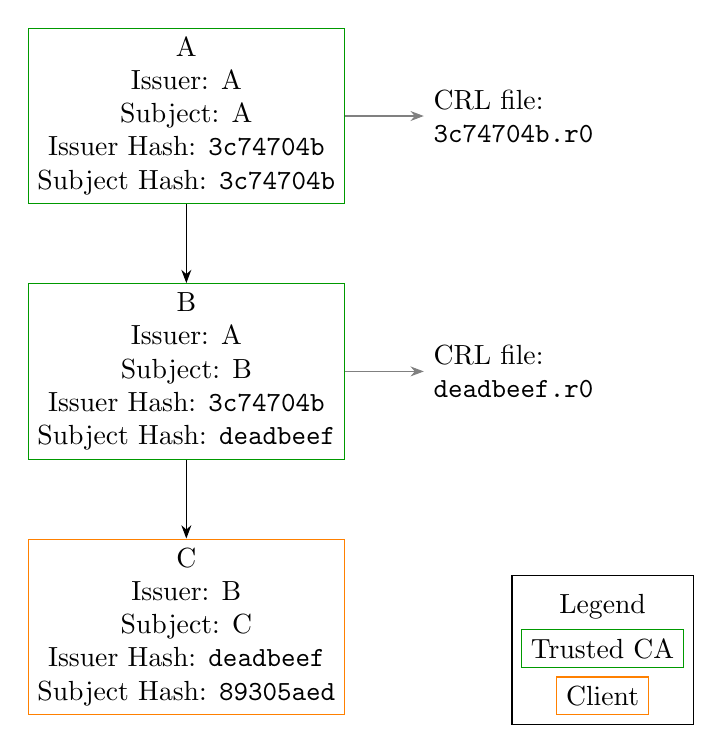
\begin{tikzpicture}
	% Styles.
	[ca/.style={rectangle,draw=green!60!black,minimum height=1cm,minimum width=1.5cm},
	leaf/.style={rectangle,draw=orange,minimum height=1cm, minimum width=1.5cm}]
	% Certificates.
	\node (A) at (0, 0) [ca,align=center] {A \\ Issuer: A \\ Subject: A \\ Issuer Hash: \texttt{3c74704b} \\ Subject Hash: \texttt{3c74704b}};
	\node (B) [below=of A] [ca,align=center] {B \\ Issuer: A \\ Subject: B \\ Issuer Hash: \texttt{3c74704b} \\ Subject Hash: \texttt{deadbeef}};
	\node (C) [below=of B] [leaf,align=center] {C \\ Issuer: B \\ Subject: C \\ Issuer Hash: \texttt{deadbeef} \\ Subject Hash: \texttt{89305aed}};
	\draw[-Stealth] (A) -- (B);
	\draw[-Stealth] (B) -- (C);
	\node (A CRL) [right=of A,align=left] {CRL file: \\ \texttt{3c74704b.r0}};
	\node (B CRL) [right=of B,align=left] {CRL file: \\ \texttt{deadbeef.r0}};
	\draw[-Stealth,gray] (A) -- (A CRL);
	\draw[-Stealth,gray] (B) -- (B CRL);
	% Legend.
	\node (lanchor) at (current bounding box.south east) {};
	\node (legend) at (lanchor) [above=1.1cm] {Legend};
	\node (l1) at (lanchor) [above=0.6cm,draw=green!60!black] {Trusted CA};
	\node (l2) at (lanchor) [above=0.0cm,draw=orange] {Client};
	\node [rectangle,draw,fit=(legend) (l1) (l2)] {};
\end{tikzpicture}
}
\end{makeimage}
\caption{Each CA requires its own CRL file.  The CRL file name is based on the hash of its issuer name.  Note that the \emph{issuer} of the CRL file is the \emph{subject} of its respective CA.}
\end{figure}
\end{center}

One more caveat: OpenSSL does not seem to report any error if the CRL path directory does not exist.  Figures.


% Syncing the Gentoo repository.
\section{2017-08-23 Securely Syncing the Gentoo Repository via a Local Server}

\begin{center}
\begin{figure}
\begin{makeimage}
\fbox{
\begin{tabular}{l|l}
Before: & After: \\
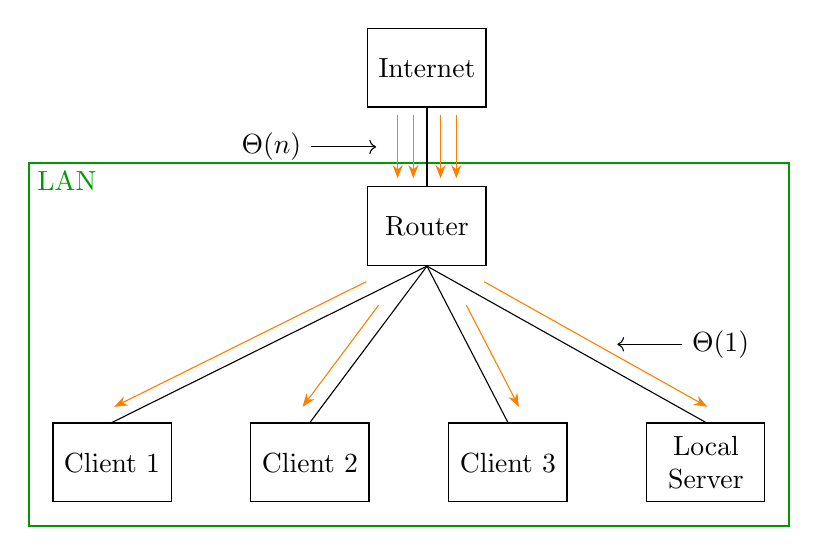
\begin{tikzpicture}
	% Machines.
	[puter/.style={rectangle,draw,minimum height=1cm,minimum width=1.5cm}]
	\node (client1)  at (0, 0) [puter] {Client 1};
	\node (client2)  [right=of client1] [puter] {Client 2};
	\node (client3)  [right=of client2] [puter] {Client 3};
	\node (server)   [right=of client3] [puter] {\parbox{1cm}{\centering Local \\ Server}};
	\node (router)   at (4, 3) [puter] {Router};
	\node (internet) [above=of router] [puter] {Internet};
	% Links.
	\draw (client1.north) -- (router.south)
		node[pos=0.1,left=0.2,circle](c1-r){}
		node[pos=0.9,left=0.2,circle](r-c1){};
	\draw (client2.north) -- (router.south)
		node[pos=0.1,left=0.07,circle](c2-r){}
		node[pos=0.75,left=0.07,circle](r-c2){};
	\draw (client3.north) -- (router.south)
		node[pos=0.1,right=0.07,circle](c3-r){}
		node[pos=0.75,right=0.07,circle](r-c3){};
	\draw (server.north) -- (router.south)
		node[pos=0.1,right=0.2,circle](s-r){}
		node[pos=0.9,right=0.2,circle](r-s){}
		node[pos=0.5,right=0.3,circle](smid){};
	\draw (router.north) -- (internet.south)
		node[pos=0.1,left=0.2,circle](r1-i1){}
		node[pos=0.1,left=0,circle](r2-i2){}
		node[pos=0.1,right=0,circle](r3-i3){}
		node[pos=0.1,right=0.2,circle](r4-i4){}
		node[pos=0.9,left=0.2,circle](i1-r1){}
		node[pos=0.9,left=0,circle](i2-r2){}
		node[pos=0.9,right=0,circle](i3-r3){}
		node[pos=0.9,right=0.2,circle](i4-r4){}
		node[pos=0.5,left=0.3,circle](mid){};
	% Traffic.
	\draw[orange,-Stealth] (r-c1.center) -- (c1-r.center);
	\draw[orange,-Stealth] (r-c2.center) -- (c2-r.center);
	\draw[orange,-Stealth] (r-c3.center) -- (c3-r.center);
	\draw[orange,-Stealth] (r-s.center) -- (s-r.center);
	\draw[orange,-Stealth] (i1-r1.center) -- (r1-i1.center);
	\draw[orange,-Stealth] (i2-r2.center) -- (r2-i2.center);
	\draw[orange,-Stealth] (i3-r3.center) -- (r3-i3.center);
	\draw[orange,-Stealth] (i4-r4.center) -- (r4-i4.center);
	\draw [<-] (mid) -- +(-1, 0) node[left]{$\Theta(n)$};
	\draw [<-] (smid) -- +(1, 0) node[right]{$\Theta(1)$};
	% LAN box.
	\begin{scope}[on background layer]
		\node (bback) [rectangle,thick,draw=green!60!black,inner sep=0.3cm,fit=(client1) (server) (router)] {};
		\node [below right,text=green!60!black] at (bback.north west) {LAN};
	\end{scope}
\end{tikzpicture}
&  % Copy+paste'd
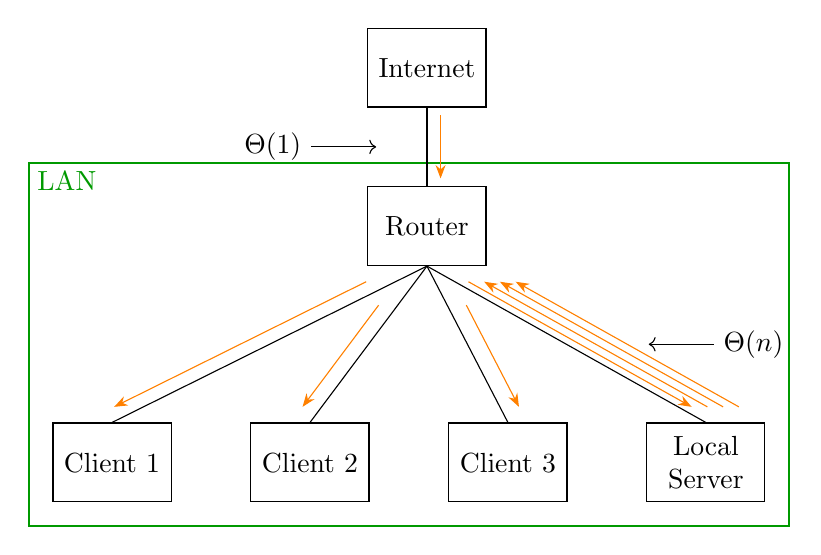
\begin{tikzpicture}
	% Machines.
	[puter/.style={rectangle,draw,minimum height=1cm,minimum width=1.5cm}]
	\node (client1)  at (0, 0) [puter] {Client 1};
	\node (client2)  [right=of client1] [puter] {Client 2};
	\node (client3)  [right=of client2] [puter] {Client 3};
	\node (server)   [right=of client3] [puter] {\parbox{1cm}{\centering Local \\ Server}};
	\node (router)   at (4, 3) [puter] {Router};
	\node (internet) [above=of router] [puter] {Internet};
	% Links.
	\draw (client1.north) -- (router.south)
		node[pos=0.1,left=0.2,circle](c1-r){}
		node[pos=0.9,left=0.2,circle](r-c1){};
	\draw (client2.north) -- (router.south)
		node[pos=0.1,left=0.07,circle](c2-r){}
		node[pos=0.75,left=0.07,circle](r-c2){};
	\draw (client3.north) -- (router.south)
		node[pos=0.1,right=0.07,circle](c3-r){}
		node[pos=0.75,right=0.07,circle](r-c3){};
	\draw (server.north) -- (router.south)
		node[pos=0.1,right=0,circle](s-r){}
		node[pos=0.9,right=0,circle](r-s){}

		node[pos=0.1,right=0.2,circle](s-c1){}
		node[pos=0.9,right=0.2,circle](c1-s){}
		node[pos=0.1,right=0.4,circle](s-c2){}
		node[pos=0.9,right=0.4,circle](c2-s){}
		node[pos=0.1,right=0.6,circle](s-c3){}
		node[pos=0.9,right=0.6,circle](c3-s){}

		node[pos=0.5,right=0.7,circle](smid){};
	\draw (router.north) -- (internet.south)
		node[pos=0.9,right=0,circle](i-s){}
		node[pos=0.1,right=0,circle](s-i){}
		node[pos=0.5,left=0.3,circle](mid){};
	% Traffic.
	\draw[orange,-Stealth] (r-c1.center) -- (c1-r.center);
	\draw[orange,-Stealth] (r-c2.center) -- (c2-r.center);
	\draw[orange,-Stealth] (r-c3.center) -- (c3-r.center);
	\draw[orange,-Stealth] (r-s.center) -- (s-r.center);
	\draw[orange,-Stealth] (s-c1.center) -- (c1-s.center);
	\draw[orange,-Stealth] (s-c2.center) -- (c2-s.center);
	\draw[orange,-Stealth] (s-c3.center) -- (c3-s.center);
	\draw[orange,-Stealth] (i-s.center) -- (s-i.center);
	\draw [<-] (mid) -- +(-1, 0) node[left]{$\Theta(1)$};
	\draw [<-] (smid) -- +(1, 0) node[right]{$\Theta(n)$};
	% LAN box.
	\begin{scope}[on background layer]
		\node (bback) [rectangle,thick,draw=green!60!black,inner sep=0.3cm,fit=(client1) (server) (router)] {};
		\node [below right,text=green!60!black] at (bback.north west) {LAN};
	\end{scope}
\end{tikzpicture}
\end{tabular}
}
\end{makeimage}
\caption{Using a local server for the Gentoo repository takes pressure off of the (often relatively slow) Internet connection and places it onto the (often relatively fast) LAN, especially important for those whose Internet is metered.}
\end{figure}
\end{center}

Running multiple Gentoo machines normally means keeping a copy of the Gentoo repository on each machine; by default this also means updating each copy of the repository by having each machine call out to the Gentoo mirrors on a regular basis for updates.  This is a waste of both local and upstream bandwidth and resources, because, within a given time period, the repository is the exact same regardless of the type of machine it is on; instead, it is more efficient to set up one machine as a server that synchronizes with upstream, then have the other local machines synchronize to said local server.  This guide will explain how to do that securely.

Though there are multiple protocols that Portage can use for synchronization, this guide will cover only SSH, and \texttt{rsync+stunnel}.  Both of these are secure, allowing synchronization over an untrusted network, albeit the local server must be trusted.  Securely syncing the server to the upstream repository with \texttt{FEATURES=webrsync-gpg} is not covered here, as it is instead covered \htmladdnormallink{here}{https://wiki.gentoo.org/wiki/Handbook:AMD64/Working/Features#Validated_Gentoo_repository_snapshots}.

\subsection{SSH Synchronization}
One of the pros of SSH-based synchronization is that it requires no extra server configuration for machines that already have SSH access to the server.  The downside is that SSH access means shell access, which might not be desirable if any of the local machines is not fully trusted, for example, because it is running proprietary applications for, say, video games; one could try and circumvent this potential security weakness by giving the SSH user a restricted shell such as \texttt{rssh}, but I was unable to get \texttt{rssh} working with the \texttt{rsync} arguments that Portage wanted to use (note: Portage calls \texttt{rsync} over the SSH session).  Thus I prefer \texttt{rsync+stunnel}, but am including the SSH method for completeness and possible future reference.
\subsubsection{Server} Assuming that \texttt{sshd} is already set up (find one of many guides if it is not), the only thing that may need to be done is to add a special user for synchronization.  In order to add the user, run
\begin{quote}
\begin{verbatim}
	# useradd -m -s /bin/bash rsyncuser
	# passwd rsyncuser
\end{verbatim}
\end{quote}
\ldots then edit the SSH daemon configuration file, usually \texttt{/etc/ssh/sshd_config}, to contain the following line:
\begin{quote}
\begin{verbatim}
	AllowUsers rsyncuser
\end{verbatim}
\end{quote}
Depending on the selected authentication method for SSH, this may be enough to give the user access; however, in the case that only key-based authentication is allowed (usually via something like \texttt{PasswordAuthentication no} \& \texttt{ChallengeResponseAuthentication no} in \texttt{sshd_config}) an SSH keypair will need to be generated for the user and the private key copied to each client that wishes to synchronize with the server.  This can be done with the following commands:
\begin{quote}
\begin{verbatim}
	# cd /home/rsyncuser
	# su rsyncuser
	$ umask 0066
	$ mkdir -p .ssh
	$ ssh-keygen -a 16 -t ed25519
	$ cp .ssh/id_ed25519.pub .ssh/authorized_keys
\end{verbatim}
\end{quote}
This will create a keypair for the \texttt{rsyncyser} and authorize that keypair for SSH login.  The \texttt{.ssh/id_ed25519} file (the private key) will then need to be copied to the client machines, probably via a USB storage device:
\begin{quote}
\begin{verbatim}
	# cp .ssh/id_ed25519 /path/to/probably/usb/storage/device
\end{verbatim}
\end{quote}

This ends the server-side configuration.

\subsubsection{Clients}
By default, Portage knows how to use SSH for synchronization, so basic setup is quite simple, although some of the details are rather esoteric.

In order to tell Portage to synchronize over SSH, if it hasn't been done already, set up the main repository configuration via:
\begin{quote}
\begin{verbatim}
	# mkdir -p /etc/portage/repos.conf
	# cp /usr/share/portage/config/repos.conf /etc/portage/repos.conf/gentoo.conf
\end{verbatim}
\end{quote}
This creates, at the time of this writing, at least, a sane configuration file for the default repository that can then be reconfigured.  With this file created, Portage should function as it always has; the defaults must be overridden in order to actually change its behavior. In order to use SSH, edit the \texttt{/etc/portage/repos.conf/gentoo.conf} file by changing the \texttt{sync-uri} option under the \texttt{[gentoo]} section to read:
\begin{quote}
\begin{verbatim}
	sync-uri = ssh://rsyncuser@192.168.1.1/usr/portage
\end{verbatim}
\end{quote}
\ldots where \texttt{192.168.1.1} is replaced with the network address of the local server.  Portage will now begin trying to sync via SSH.

"Trying" may be the modus operandi depending on whether or not the local server strictly requires keys or will accept user passwords; it is thus useful to understand where Portage stores its SSH information, as its home directory is not \texttt{/home/portage}, but, as \texttt{/etc/passwd} reveals, \texttt{/var/tmp/portage}, thus SSH configuration goes into \texttt{/var/tmp/portage/.ssh}.  In order to get Portage to use \texttt{rsyncuser}'s key, run the following:
\begin{quote}
\begin{verbatim}
	# mkdir -p /var/tmp/portage/.ssh
	# umask 0066
	# cp /path/from/probably/usb/device/with/rsyncusers/key/id_ed25519 /var/tmp/portage/.ssh/id_ed25519
	# chown -R portage:portage /var/tmp/portage/.ssh
\end{verbatim}
\end{quote}
Portage should now pickup \texttt{rsyncuser}'s key when it tries to synchronize.

Admittedly, storing valuable authentication information in a \texttt{/var/tmp} subdirectory seems risky at best.  Another option for storing the key is to place the key at a more stable location and then tell Portage where to find it.  Start by placing the key somewhere safer:
\begin{quote}
\begin{verbatim}
	# mkdir -p /usr/local/portage/.ssh
	# chmod 700 /usr/local/portage/.ssh
	# chown -R portage:portage /usr/local/portage/.ssh
	# mv /var/tmp/portage/.ssh/id_ed25519 /usr/local/portage/.ssh/
\end{verbatim}
\end{quote}
\ldots then tell Portage where to find the key by adding the following line to \texttt{/etc/portage/make.conf}:
\begin{quote}
\begin{verbatim}
	PORTAGE_SSH_OPTS="-i /usr/local/portage/.ssh/id_ed25519"
\end{verbatim}
\end{quote}
Portage will now look for the \texttt{rsyncuser}'s key at the previously-specified location.

This solves the \texttt{rsyncuser}'s key problem, but what about the important \texttt{known_hosts} file?  Well, I didn't get that far.  I don't fully trust of all my machines, and do not want to give all of them shell access to my server, and, since I couldn't get \texttt{rssh} to work with Portage and was looking for an excuse to play with \texttt{stunnel}, I decided to work on it instead, thus \texttt{rsync+stunnel} is the topic of the next section.

\subsection{Rsync+stunnel Synchronization}
This method works by using an \texttt{rsync} daemon to synchronize between the local server and client; however, because \texttt{rsync} is unencrypted, the connection is wrapped via the \texttt{stunnel} daemon, which uses \htmladdnormallink{TLS}{https://en.wikipedia.org/wiki/Transport_Layer_Security} for encryption and authentication.  \texttt{stunnel} must be configured on both the local server and each client.

\subsubsection{Server}
Start by setting up the \texttt{rsync} daemon without \texttt{stunnel}.  By default, Gentoo comes with a disabled but sane configuration file at \texttt{/etc/rsyncd.conf}.  Adding a few extra lines gives, excluding comments, the following:
\begin{quote}
\begin{verbatim}
	pid file = /run/rsyncd.pid
	use chroot = yes
	read only = yes
	hosts allow = 192.168.1.1/16
	reverse lookup = no
	timeout = 60

	[gentoo-portage]
	path = /usr/portage
	comment = Gentoo Portage tree
	exclude = /distfiles /packages
\end{verbatim}
\end{quote}
By default this configuration file creates an \texttt{rsync} \textit{module} that clients can synchronize with; this module is read-only and excludes directories that are not a part of the repository.  The extra options are: \texttt{hosts allow = 192.168.1.1/16}, which tells \texttt{rsync} to only accept connections from hosts in the specified block and must be appropriate to the local network; \texttt{reverse lookup = no}, which disables reverse-DNS lookups of client IP addresses; and \texttt{timeout = 60}, which sets a small timeout for unresponsive clients.  See \texttt{man 5 rsyncd.conf} for details; the extra options are not strictly necessary for the purposes of this guide.

The next step is to install and configure \texttt{stunnel}.  This involves four steps: installing the program, configuring the service, generating certificates, and creating the service: To install \texttt{stunnel}, run:
\begin{quote}
\begin{verbatim}
	# emerge -av stunnel
\end{verbatim}
\end{quote}
For convenience, the Gentoo developers created a useful example configuration file for \texttt{rsync+stunnel} which may be installed by running:
\begin{quote}
\begin{verbatim}
	USE="stunnel" emerge -av rsync
\end{verbatim}
\end{quote}
This creates the file \texttt{/etc/stunnel/rsyncd.conf}.  Move it to \texttt{/etc/stunnel/rsyncd-stunnel.conf} for \texttt{init} scripts (later), and reconfigure it such that, excluding comments, it has the following options:
\begin{quote}
\begin{verbatim}
	foreground = no
	pid = /var/run/stunnel/rsyncd-stunnel.pid
	socket = l:TCP_NODELAY=1
	socket = r:TCP_NODELAY=1
	setuid = root
	setgid = root

	[rsync]
	accept = 874
	cert = /etc/stunnel/rsyncd-stunnel.crt
	key  = /etc/stunnel/rsyncd-stunnel.key
	client = no

	exec = /usr/bin/rsync
	execargs = rsync --server --daemon --config=/etc/rsyncd.conf .
\end{verbatim}
\end{quote}
Most of these options come with the default configuration file, but make sure to change the \texttt{pid} option.  The \texttt{cert} and \texttt{key} options specify where the \htmladdnormallink{X.509}{https://en.wikipedia.org/wiki/X.509} certificate and its key are to be loaded from (they will be generated later).  Port \texttt{874} is used in place of \texttt{873}, as it is not a plaintext \texttt{rsync} service.  Client verification is not wanted here, so make sure to remove any \texttt{verify} and \texttt{CAfile} lines.

In order to generate the server's certificate, run the following series of commands:
\begin{quote}
\begin{verbatim}
	# cd /etc/stunnel
	# umask 0077
	# openssl genrsa -out rsyncd-stunnel.key 4096
	# openssl req -key rsyncd-stunnel.key -new -x509 -days 7200 -sha512 -out rsyncd-stunnel.crt -subj '/CN=rsyncd-stunnel/'
\end{verbatim}
\end{quote}
The short story here is that this will create a certificate and key pair for TLS that will last for almost 20 years, see \texttt{man genrsa} and \texttt{man req} for details.

Finally, create the service with:
\begin{quote}
\begin{verbatim}
	# cd /etc/init.d
	# ln -s stunnel rsyncd-stunnel
\end{verbatim}
\end{quote}
This uses the default \texttt{stunnel} init script, except it will look for a configuration file at \texttt{/etc/stunnel/rsyncd-stunnel.conf}, hence the earlier renaming that was done.  To start the service, run \texttt{rc-service rsyncd-stunnel start}, and don't forget to add it to the default runlevel via:
\begin{quote}
\begin{verbatim}
	# rc-update add rsyncd-stunnel default
\end{verbatim}
\end{quote}

The server should now be configured and ready for synchronization.  The clients must now be configured to trust and use the server.

\subsubsection{Clients}
The client must now be configured so that when Portage attempts to sync it will use the secure connection \textbf{and} it will validate that it is syncing with the server, otherwise a malicious actor could imitate the server and send a compromised repository.  This involves installing and configuring \texttt{stunnel}, configuring Portage, then creating the service.

Begin by installing \texttt{stunnel}:
\begin{quote}
\begin{verbatim}
	# emerge -av stunnel
\end{verbatim}
\end{quote}
\ldots then configure \texttt{stunnel} so that, without comments, the configuration file \texttt{/etc/stunnel/stunnel.conf} reads:
\begin{quote}
\begin{verbatim}
	setuid = stunnel
	setgid = stunnel
	pid = /run/stunnel/stunnel.pid
	socket = l:TCP_NODELAY=1
	socket = r:TCP_NODELAY=1

	[rsync-stunnel]
	client     = yes
	CAfile     = /etc/stunnel/rsyncd-stunnel.crt
	verifyPeer = yes
	accept     = 127.0.0.1:873
	connect    = 192.168.1.200:874
\end{verbatim}
\end{quote}
This creates an \texttt{stunnel} \emph{service}.  The \texttt{client} argument lets \texttt{stunnel} know to run \texttt{rsync} as a client rather than as a server.  The \texttt{CAfile} argument specifies the location of the server certificate to use (note that it has not yet been copied over to the client).  The \texttt{verifyPeer} is especially important as enabling it will actually validate the server certificate; without this enabled a malicious actor could intercept and modify the traffic.  The \texttt{accept} argument specifies where the \texttt{stunnel} program will listen for client connections, Portage will later be configured to make connections here.  The \texttt{connect} argument specifies where the \texttt{stunnel} program will connect to; it must be set to the address and port of the local server.  The other options are fairly standard.  Note that, unlike the server, this setup is using the default \texttt{stunnel} settings, configuring multiple \texttt{stunnel} services at the OpenRC level would require modifying a few parameters, such as the PID (Process ID) and the filename of the configuration.

Now that \texttt{stunnel} has been configured, make sure to copy the certificate from the local server to the client.  This should be done via a trusted storage device (USB stick, SD Card, \&c.) or the certificate retrieved via a command such as OpenSSL's \texttt{s\_client} (usage not covered here) and its fingerprint manually verified.
\begin{quote}
\begin{verbatim}
	# cp /path/from/secure/storage/device /etc/stunnel/rsyncd-stunnel.crt
\end{verbatim}
\end{quote}
\texttt{stunnel} now has all that it needs to securely tunnel a connection to the server.

Portage must now be configured to use the secure tunnel.  As with SSH configuration, begin by overriding the default repository configuration:
\begin{quote}
\begin{verbatim}
	# mkdir -p /etc/portage/repos.conf
	# cp /usr/share/portage/config/repos.conf /etc/portage/repos.conf/gentoo.conf
\end{verbatim}
\end{quote}
\ldots then modify the \texttt{sync-uri} argument to correspond to the \texttt{accept} argument configured in \texttt{stunnel}:
\begin{quote}
\begin{verbatim}
	sync-uri = rsync://127.0.0.1:873/gentoo-portage
\end{verbatim}
\end{quote}
This will synchronize with the \texttt{gentoo-portage} module defined on the local server's \texttt{/etc/rsyncd.conf}.  Note how the use of \texttt{stunnel} is completely transparent to Portage.  This has the minor disadvantage that error diagnostics must be found in log message from \texttt{stunnel} and not the Portage frontend, but is usually not a problem once things have been configured properly.

Next, start the service and add it to the default runlevel:
\begin{quote}
\begin{verbatim}
	# rc-service stunnel start
	# rc-update add stunnel default
\end{verbatim}
\end{quote}
\ldots then try it out with:
\begin{quote}
\begin{verbatim}
	# emerge --sync
\end{verbatim}
\end{quote}
Portage should now be securely synchronizing to the local server!  Repeat these steps for each client that needs to synchronize with the local server.


% Ancient Apparition Bowling
\section{2017-07-17 Ancient Apparition Bowling}
This is a silly metagame that I came up with for a DotA2 custom game.  It may not be possible to beat, but I've yet to try all strategies.

\subsection*{Origin}
Mercilessly slaughtering bots using weird combinations of cheats in DotA2 is an easy way to blow off a little steam after a difficult match.  One day I decided to go "bowling" with Ancient Apparition; I'd cheat to maximum level, 6-slot, enable wtf mode, and snipe the bots from base with his ultimate.
This is loads of fun, until the creeps start pushing towers, at which point the bots also take advantage of wtf mode and begin spamming fortify, leading to a frustrating stalemate.  The workaround for this is to disable wtfmode and instead use the \texttt{-refresh} cheat, which, although it does reset fortify cooldowns, can be used in conjunction with a Refresher Orb to blast the bots with two ultimates while giving them only one fortify.

The result is a semi-functional slaughtering of bots, although having to constantly open the command prompt to paste and submit the \texttt{-refresh} command gets annoying after a while; sadly, there doesn't seem to be a way to disable the bots' fortify spam.  After a little bit of this, I noticed that the cooldown of the metaphorical bowling ball and the travel time were not that far apart, leading me to wonder if I could play this game successfully without having to spam cheat commands (and reset the fortify cooldown) all game long.  Thus "Ancient Apparition Bowling" was born.

\subsection*{Rules}
These are the rules of the game, and though they may not be comprehensive, you should be able to understand the jist of them.  First, stay in fountain for the duration of the match.  Second, use cheats to give yourself max level (\texttt{-lvlup 25}), 6-slots (\texttt{-item <name>}), and vision (\texttt{-allvision}).  Third, no backpack, stash, or other item-use shenanegains; stick to your 6 slots.  Fourth, no bots on your team and five bots of highest difficulty on the other team.  That's it!
\begin{figure}
\includegraphics[scale=0.33]{files/blog/2017_07_17_ancient_apparition_bowling/fountain.png}
\caption{Where you will be spending all of your time.}
\end{figure}

Your goal is now to destroy the bots' ancient before the bots level up enough to tank through your ult and push your base.  This is more difficult than it sounds, as the bots are actually rather crafty and level up sooner than you might expect.

\subsection*{Strategy}
My current build involves getting an Aghaim's Scepter, Octarine Core, Refresher Orb, and 3 Aether Lens.  Perhaps you can think up something better.
\begin{figure}
\includegraphics{files/blog/2017_07_17_ancient_apparition_bowling/items.png}
\end{figure}

It is difficult to push all lanes at once, since the bots can quickly respawn at lower levels, and you only have so many ultimates to shoot off.  It would thus seem prudent to choose a particular lane to hammer, but how to do so isn't actually obvious.

The strategy that I tried was to focus the enemy creeps at their spawning point in a side lane.  This can be done by firing consistently at the 18 and 48 second marks towards the front of their 3rd tower. This will obliterate all of the creeps during the early part of the game.  Make sure to adjust your ultimate slightly to the left each time in order to adjust for the micro-delay between your ult going off cooldown and actually launching your ult; you can reset this after a while with a Refresher Orb.
\begin{figure}
\includegraphics[scale=0.33]{files/blog/2017_07_17_ancient_apparition_bowling/towerhit.png}
\caption{Killing creeps as soon as they spawn.}
\end{figure}

Though this may at first seem like a good way to get the creeps to push the tower, the bots are actually crafty enough to pull the creeps behind the tower, limiting the amount of damage done.  While I was able to eventually push to their barracks, at this point the other bots also helped pull the creeps behind the barracks, and eventually became strong enough to tank the ult and push my base, thus making this a losing strategy.
\begin{figure}
\includegraphics[scale=0.33]{files/blog/2017_07_17_ancient_apparition_bowling/botpull.png}
\caption{Sneaky bots pulling creeps away from the tower.}
\end{figure}

A possible variation would be to try focusing down the bots themselves, but this is tricky as they often move out of the ult's way.  A hybrid combination may involve finding a position where the bots and creeps are likely to align, then aiming to kill the creeps and probably the bots.  It may also be easier to push straight up middle rather than taking out a side lane first, especially as the bots seem found of charging up mid.

I've yet to win at this metagame.  It might not even be plausible.  Try it yourself and see what happens!

\subsection*{Addendum}
Between inventing this game, writing this article, and getting the screenshots, the bot fortify spam in wtf mode seems to have stopped.

\end{document}
